%%%%%%%%%%%%%%%%%%%%% chapter.tex %%%%%%%%%%%%%%%%%%%%%%%%%%%%%%%%%
%
% sample chapter
%
% Use this file as a template for your own input.
%
%%%%%%%%%%%%%%%%%%%%%%%% Springer-Verlag %%%%%%%%%%%%%%%%%%%%%%%%%%
%\motto{Use the template \emph{chapter.tex} to style the various elements of your chapter content.}

\chapter{Rosetta Code Tasks starting with S}

\section*{S-Expressions}

\href{http://en.wikipedia.org/wiki/S-Expression}{S-Expressions} are one
convenient way to parse and store data.

Write a simple reader and writer for S-Expressions that handles quoted
and unquoted strings, integers and floats.

The reader should read a single but nested S-Expression from a string
and store it in a suitable datastructure (list, array, etc). Newlines
and other whitespace may be ignored unless contained within a quoted
string. ``\texttt{()}'' inside quoted strings are not interpreted, but
treated as part of the string. Handling escaped quotes inside a string
is optional; thus ``\texttt{(foo"bar)}'' maybe treated as a string
``\texttt{foo"bar}'', or as an error.

For this, the reader need not recognise ``\texttt{\textbackslash{}}''
for escaping, but should, in addition, recognize numbers if the language
has appropriate datatypes.

Languages that support it may treat unquoted strings as symbols.

Note that with the exception of ``\texttt{()"}''
(``\texttt{\textbackslash{}}'' if escaping is supported) and whitespace
there are no special characters. Anything else is allowed without

The reader should be able to read the following input

\begin{verbatim}
((data "quoted data" 123 4.5)
 (data (!@# (4.5) "(more" "data)")))
\end{verbatim}

and turn it into a native datastructure. (see the \hyperref[Pike]{Pike},
\hyperref[Python]{Python} and \hyperref[Ruby]{Ruby} implementations for
examples of native data structures.)

The writer should be able to take the produced list and turn it into a
new S-Expression. Strings that don't contain whitespace or parentheses
() don't need to be quoted in the resulting S-Expression, but as a
simplification, any string may be quoted.



\begin{wideverbatim}

The '[http://software-lab.de/doc/refA.html#any any]' function parses an
s-expression from a string (indentical to the way
'[http://software-lab.de/doc/refR.html#read read]' does this from an input
stream).

: (any "((data \"quoted data\" 123 4.5) (data (!@# (4.5) \"(more\" \"data)\")))")
-> ((data "quoted data" 123 5) (data (!@# (5) "(more" "data)")))

: (view @)
+---+-- data
|   |
|   +-- "quoted data"
|   |
|   +-- 123
|   |
|   +-- 5
|
+---+-- data
    |
    +---+-- !@#
        |
        +---+-- 5
        |
        +-- "(more"
        |
        +-- "data)"

Implementing a subset of 'any' explicitly:

(de readSexpr ()
   (case (skip)
      ("(" (char) (readList))
      ("\"" (char) (readString))
      (T (readAtom)) ) ) )

(de readList ()
   (make
      (loop
         (NIL (skip))
         (T (= @ ")") (char))
         (link (readSexpr)) ) ) )

(de readString ()
   (pack
      (make
         (until (= "\"" (or (peek) (quit "Unterminated string")))
            (link (char)) )
         (char) ) ) )

(de readAtom ()
   (let X
      (make
         (until (or (sp? (peek)) (member (peek) '("(" ")")))
            (link (char)) ) )
      (or (format X) (intern (pack X))) ) )

\end{wideverbatim}

\begin{wideverbatim}

It can be used in a pipe to read from a string:

: (pipe (prin "((data \"quoted data\" 123 4.5)
                (data (!@# (4.5)\"(more\" \"data)\")))")(readSexpr))
-> ((data "quoted data" 123 5) (data (!@# (5) "(more" "data)")))

'[http://software-lab.de/doc/refS.html#sym sym]' does the reverse (i.e. builds a
symbol (string) from an expression).

: (sym @@)
-> "((data \"quoted data\" 123 5) (data (!@# (5) \"(more\" \"data)\")))"

Implementing a subset of the built-in printer:

(de printSexpr (Expr Fun)
   (cond
      ((pair Expr)
         (Fun "(")
         (printSexpr (car Expr) Fun)
         (for X (cdr Expr)
            (Fun " ")
            (printSexpr X Fun) )
         (Fun ")") )
      ((str? Expr)
         (Fun "\"")
         (mapc Fun (chop Expr))
         (Fun "\"") )
      (T (mapc Fun (chop Expr))) ) )

This can be used for plain printing

: (printSexpr
   '((data "quoted data" 123 4.5) (data (!@# (4.5) "(more" "data)")))
   prin )
((data "quoted data" 123 5) (data (!@# (5) "(more" "data)")))

or to collect the characters into a string:

: (pack
   (make
      (printSexpr
         '((data "quoted data" 123 4.5) (data (!@# (4.5) "(more" "data)")))
         link ) ) )
-> "((data \"quoted data\" 123 5) (data (!@# (5) \"(more\" \"data)\")))"

\end{wideverbatim}

\pagebreak{}
\section*{SEDOLs}

For each number list of \textbf{6}-digit
\href{http://en.wikipedia.org/wiki/SEDOL}{SEDOLs}, calculate and
append the checksum digit.

That is, given this input:

\begin{verbatim}
710889
B0YBKJ
406566
B0YBLH
228276
B0YBKL
557910
B0YBKR
585284
B0YBKT
B00030
\end{verbatim}

Produce this output:

\begin{verbatim}
7108899
B0YBKJ7
4065663
B0YBLH2
2282765
B0YBKL9
5579107
B0YBKR5
5852842
B0YBKT7
B000300
\end{verbatim}

For extra credit, check each input is correctly formed, especially with
respect to valid characters allowed in a SEDOL string.

C.f. \emph{Luhn test}


\begin{wideverbatim}

(de sedol (Str)
   (pack Str
      (char
         (+ `(char "0")
            (\%
               (- 10
                  (\%
                     (sum
                        '((W C)
                           (cond
                              ((>= "9" C "0")
                                 (* W (format C)) )
                              ((>= "Z" (setq C (uppc C)) "A")
                                 (* W (+ 10 (- (char C) `(char "A")))) ) ) )
                        (1 3 1 7 3 9)
                        (chop Str) )
                     10 ) )
               10 ) ) ) ) )

(for S '("710889" "B0YBKJ" "406566" "B0YBLH" "228276" "B0YBKL"
           "557910" "B0YBKR" "585284" "B0YBKT" "B00030" )
   (prinl (sedol S)) )

\end{wideverbatim}

\pagebreak{}
\section*{SHA-1}

\textbf{SHA-1} or \textbf{SHA1} is a one-way hash function; it computes
a 160-bit message digest. SHA-1 often appears in security protocols; for
example, many HTTPS websites use RSA with SHA-1 to secure their
connections. BitTorrent uses SHA-1 to verify downloads. Git and
Mercurial use SHA-1 digests to identify commits.

A US government standard,
\href{http://www.itl.nist.gov/fipspubs/fip180-1.htm}{FIPS 180-1},
defines SHA-1.

Find the SHA-1 message digest for a string of
\emph{octets}. You may either call a SHA-1 library, or
implement SHA-1 in your language. Both approaches interest Rosetta Code.


\begin{wideverbatim}

(let Str "Rosetta Code"
   (pack
      (mapcar '((B) (pad 2 (hex B)))
         (native "libcrypto.so" "SHA1" '(B . 20) Str (length Str) '(NIL (20))) ) ) )

Output:

-> "48C98F7E5A6E736D790AB740DFC3F51A61ABE2B5"

\end{wideverbatim}

\pagebreak{}
\section*{Safe addition}

Implementation of
\href{http://en.wikipedia.org/wiki/Interval\_arithmetic}{interval
  arithmetic} and more generally fuzzy number arithmetic require
operations that yield safe upper and lower bounds of the exact result.
For example, for an addition, it is the operations *↑ and *↓ defined
as: \emph{a} +↓ \emph{b} ≤ \emph{a} + \emph{b} ≤ \emph{a} +↑ \emph{b}.
Additionally it is desired that the width of the interval (\emph{a} +↑
\emph{b}) - (\emph{a} +↓ \emph{b}) would be about the machine epsilon
after removing the exponent part.

Differently to the standard floating-point arithmetic, safe interval
arithmetic is \textbf{accurate} (but still imprecise). I.e. the result
of each defined operation contains (though does not identify) the exact
mathematical outcome.

Usually a
\href{http://en.wikipedia.org/wiki/Floating\_Point\_Unit}{FPU's} have
machine +,-,*,/ operations accurate within the machine precision. To
illustrate it, let us consider a machine with decimal floating-point
arithmetic that has the precision is 3 decimal points. If the result of
the machine addition is 1.23, then the exact mathematical result is
within the interval {]}1.22, 1.24{[}. When the machine rounds towards
zero, then the exact result is within {[}1.23,1.24{[}. This is the basis
for an implementation of safe addition.

\begin{wideverbatim}

PicoLisp uses scaled integer arithmetics, with unlimited precision, for all
operations on real numbers. For that reason addition and subtraction are always
exact. Multiplication is also exact (unless the result is explicitly scaled by
the user), and division in combination with the remainder.

\end{wideverbatim}

\pagebreak{}
\section*{Same Fringe}

Write a routine that will compare the leaves (``fringe'') of two binary
trees to determine whether they are the same list of leaves when visited
left-to-right. The structure or balance of the trees does not matter;
only the number, order, and value of the leaves is important.

Any solution is allowed here, but many computer scientists will consider
it inelegant to collect either fringe in its entirety before starting to
collect the other one. In fact, this problem is usually proposed in
various forums as a way to show off various forms of concurrency
(tree-rotation algorithms have also been used to get around the need to
collect one tree first). Thinking of it a slightly different way, an
elegant solution is one that can perform the minimum amount of work to
falsify the equivalence of the fringes when they differ somewhere in the
middle, short-circuiting the unnecessary additional traversals and
comparisons.

Any representation of a binary tree is allowed, as long as the nodes are
orderable, and only downward links are used (for example, you may not
use parent or sibling pointers to avoid recursion).

\begin{wideverbatim}


This uses coroutines to traverse the trees, so it works only in the
64-bit version.

(de nextLeaf (Rt Tree)
   (co Rt
      (recur (Tree)
         (when Tree
            (recurse (cadr Tree))
            (yield (car Tree))
            (recurse (cddr Tree)) ) ) ) )
 
(de cmpTrees (Tree1 Tree2)
   (prog1
      (use (Node1 Node2)
         (loop
            (setq
               Node1 (nextLeaf "rt1" Tree1)
               Node2 (nextLeaf "rt2" Tree2) )
            (T (nor Node1 Node2) T)
            (NIL (= Node1 Node2)) ) )
      (co "rt1")
      (co "rt2") ) )

\end{wideverbatim}

\begin{wideverbatim}

Test:

: (balance '*Tree1 (range 1 7))
-> NIL
: (for N (5 4 6 3 7 1 2) (idx '*Tree2 N T))
-> NIL
 
: (view *Tree1 T)
      7
   6
      5
4
      3
   2
      1
-> NIL
 
: (view *Tree2 T)
      7
   6
5
   4
      3
            2
         1
-> NIL
 
: (cmpTrees *Tree1 *Tree2)
-> T

\end{wideverbatim}

\pagebreak{}
\section*{Scope modifiers}

Most programming languages offer support for
\emph{subroutines}. When execution changes
between subroutines, different sets of variables and functions
(``scopes'') are available to the program. Frequently these sets are
defined by the placement of the variable and function declarations
(``static scoping'' or ``lexical scoping''). These sets may also be
defined by special modifiers to the variable and function declarations.

Show the different scope modifiers available in your language and
briefly explain how they change the scope of their variable or function.
If your language has no scope modifiers, note it.


\begin{wideverbatim}


  PicoLisp distinguishes between "scope" and "binding". The scope of a
  symbol determines its visibility in a given context (whether or not
  it can be accessed), while binding is about assigning it a value.

# Scope

In PicoLisp, the scope type of a symbol is either "internal",
"transient" or "external". It is specified lexically: Internal symbols
are just normal symbols. Transient symbols are surrounded by double
quotes (and thus look like strings in other languages), and/or with an
underlined font if possible. External symbols are surrounded by
braces.

* The scope of an internal symbol is global. This means that a symbol
like AB123 is always the same object, residing at a certain location
in memory (pointer equality).

* A transient symbol like "AB123" is the same only within the current
transient scope. This is normally a single source file, but may be
further subdivided. Within that scope it can be used like an internal
symbol, but after the transient scope is closed it cannot be accessed
by its name any longer. This behavior is similar to "static"
identifiers in the C language.

* External symbols like {AB123} are persistent database symbols. They
have a permanent identity among different processes and over time.
Besides that, they have the same structure like internal and transient
symbols: A value, properties and a name.

# Binding

Regardless of the scope, the binding of symbols to values is always
dynamic. This happens implicitly for function parameters, or
explicitly with functions like
[http://software-lab.de/doc/refL.html#let let],
[http://software-lab.de/doc/refU.html#use use],
[http://software-lab.de/doc/refB.html#bind bind],
[http://software-lab.de/doc/refJ.html#job job] and others. This means
that the current value of a symbol is saved locally, then set to the
new value. When done, the old value is restored. Closures are created
by maintaining an explicit environment. More about that
[http://software-lab.de/doc/faq.html#dynamic here].

\end{wideverbatim}

\pagebreak{}
\section*{Script name}
[aka 'Program name']

The task is to programmatically obtain the name used to invoke the
program. (For example determine whether the user ran ``python
hello.py'', or ``python hellocaller.py'', a program importing the code
from ``hello.py''.)

Sometimes a \emph{multiline shebang} is necessary in order to provide
the script name to a language's internal ARGV.

See also \emph{Command-line arguments}

Examples from \href{https://github.com/mcandre/scriptname}{GitHub}.

\begin{wideverbatim}

The function '[http://software-lab.de/doc/refC.html#cmd cmd]' returns the
command name.

: (cmd)
-> "/usr/bin/picolisp"

\end{wideverbatim}

\pagebreak{}
\section*{Scripted Main}

It is useful to be able to execute a main() function only when a program
is run directly. This is a central feature in programming scripts; the
feature is called \emph{scripted main}.

Examples from \href{https://github.com/mcandre/scriptedmain}{GitHub}.

Sometimes getting the \emph{ScriptName} is required in order to
determine when to run main().

\begin{wideverbatim}

PicoLisp normally does it the other way round: It calls main from the command
line with the '-' syntax if desired. Create an executable file (chmod +x)
"life.l":

#!/usr/bin/picolisp /usr/lib/picolisp/lib.l

(de meaningOfLife ()
   42 )

(de lifemain ()
   (prinl "Main: The meaning of life is " (meaningOfLife))
   (bye) )

and an executable file (chmod +x) "test.l":

#!/usr/bin/picolisp /usr/lib/picolisp/lib.l

(load "life.l")

(prinl "Test: The meaning of life is " (meaningOfLife))
(bye)

Test:

\$ ./life.l -lifemain
Main: The meaning of life is 42

\$ ./test.l
Test: The meaning of life is 42

\end{wideverbatim}

\pagebreak{}
\section*{Search a list}

Find the index of a string (needle) in an indexable, ordered
collection of strings (haystack). Raise an exception if the needle is
missing. If there is more than one occurrence then return the smallest
index to the needle.

As an extra task, return the largest index to a needle that has multiple
occurrences in the haystack.

\begin{wideverbatim}

Note that in PicoLisp all indexes are one-based
(the first element has the position '1')

(de lastIndex (Item Lst)
   (- (length Lst) (index Item (reverse Lst)) -1) )

(de findNeedle (Fun Sym Lst)
   (prinl Sym " " (or (Fun Sym Lst) "not found")) )

(let Lst '(Zig Zag Wally Ronald Bush Krusty Charlie Bush Bozo)
   (findNeedle index 'Washington Lst)
   (findNeedle index 'Bush Lst)
   (findNeedle lastIndex 'Bush Lst) )

Output:

Washington not found
Bush 5
Bush 8

\end{wideverbatim}

\pagebreak{}
\section*{Secure temporary file}

Create a temporary file, \textbf{securely and exclusively} (opening it
such that there are no possible \emph{race
conditions}). It's fine assuming local filesystem semantics (NFS or
other networking filesystems can have signficantly more complicated
semantics for satisfying the ``no race conditions'' criteria). The
function should automatically resolve name collisions and should only
fail in cases where permission is denied, the filesystem is read-only or
full, or similar conditions exist (returning an error or raising an
exception as appropriate to the language/environment).


\begin{wideverbatim}

The 'tmp' function returns temporary file names which are exclusively for the
current process (based on the process ID). These files are automatically deleted
upon process termination. Background tasks within a single PicoLisp process is
always non-preemptive, therefore dedicated locks are usually not necessary. If
they are (e.g. because such a file name is passed to a child process), explicit
locks with the 'ctl' functions are possible.

: (out (tmp "foo") (println 123))         # Write tempfile
-> 123

: (in (tmp "foo") (read))                 # Read tempfile
-> 123

: (let F (tmp "foo")
   (ctl F                                 # Get exclusive lock
      (let N (in F (read))                # Atomic increment
         (out F (println (inc N))) ) ) )
-> 124

\end{wideverbatim}

\pagebreak{}
\section*{Self-describing numbers}

There are several integers numbers called ``self-describing'' or
"\href{http://en.wikipedia.org/wiki/Self-descriptive\_number}{self-descriptive}"

Integers with the property that, when digit positions are labeled 0 to
N-1, the digit in each position is equal to the number of times that
that digit appears in the number.

For example 2020 is a four digit self describing number.

Position ``0'' has value 2 and there is two 0 in the number. Position
``1'' has value 0 because there are not 1's in the number. Position
``2'' has value 2 and there is two 2. And the position ``3'' has value 0
and there are zero 3's.

Self-describing numbers \textless{} 100.000.000: 1210 - 2020 - 21200 -
3211000 - 42101000

Task Description

\begin{enumerate}
\item
  Write a function/routine/method/\ldots{} that will check whether a
  given positive integer is self-describing.
\item
  As an optional stretch goal - generate and display the set of
  self-describing numbers.
\end{enumerate}



\begin{wideverbatim}

(de selfDescribing (N)
   (not
      (find '((D I) (<> D (cnt = N (circ I))))
         (setq N (mapcar format (chop N)))
         (range 0 (length N)) ) ) )

Output:

: (filter selfDescribing (range 1 4000000))
-> (1210 2020 21200 3211000)

\end{wideverbatim}

\pagebreak{}
\section*{Self-referential sequence}

There are several ways to generate a self-referential sequence. One very
common one (the \emph{Look-and-say
sequence}) is to start with a positive integer, then generate the next
term by concatenating enumerated groups of adjacent alike digits:

0, 10, 1110, 3110, 132110, 1113122110, 311311222110 \ldots{}

The terms generated grow in length geometrically and never converge.

Another way to generate a self-referential sequence is to summarize the
previous term.

Count how many of each alike digit there is, then concatenate the sum
and digit for each of the sorted enumerated digits. Note that the first
five terms are the same as for the previous sequence.

0, 10, 1110, 3110, 132110, 13123110, 23124110 \ldots{} see
\href{http://oeis.org/A036058}{The On-Line Encyclopedia of Integer
Sequences}

Sort the digits largest to smallest. Do not include counts of digits
that do not appear in the previous term.

Depending on the seed value, series generated this way always either
converge to a stable value or to a short cyclical pattern. (For our
purposes, I'll use converge to mean an element matches a previously seen
element.) The sequence shown, with a seed value of 0, converges to a
stable value of 1433223110 after 11 iterations. The seed value that
converges most quickly is 22. It goes stable after the first element.
(The next element is 22, which has been seen before.)

\pagebreak{}
\textbf{Task:}

Find all the positive integer seed values under 1000000, for the above
convergent self-referential sequence, that takes the largest number of
iterations before converging. Then print out the number of iterations
and the sequence they return. Note that different permutations of the
digits of the seed will yield the same sequence. For this task, assume
leading zeros are not permitted.

\begin{wideverbatim}
Seed Value(s): 9009 9090 9900

Iterations: 21 

Sequence: (same for all three seeds except for first element)
9009
2920
192210
19222110
19323110
1923123110
1923224110
191413323110
191433125110
19151423125110
19251413226110
1916151413325110
1916251423127110
191716151413326110
191726151423128110
19181716151413327110
19182716151423129110
29181716151413328110
19281716151423228110
19281716151413427110
19182716152413228110
\end{wideverbatim}

See also: \emph{Self-describing numbers} and \emph{Look-and-say
  sequence}


\begin{wideverbatim}

Using 'las' from [[Look-and-say sequence#PicoLisp]]:

(de selfRefSequence (Seed)
   (let L (mapcar format (chop Seed))
      (make
         (for (Cache NIL  (not (idx 'Cache L T)))
            (setq L
               (las (flip (sort (copy (link L))))) ) ) ) ) )

(let Res NIL
   (for Seed 1000000
      (let N (length (selfRefSequence Seed))
         (cond
            ((> N (car Res)) (setq Res (list N Seed)))
            ((= N (car Res)) (queue 'Res Seed)) ) ) )
   (println 'Values: (cdr Res))
   (println 'Iterations: (car Res))
   (mapc prinl (selfRefSequence (cadr Res))) )

Output:

Values: (9009 9090 9900)
Iterations: 21
9009
2920
192210
19222110
19323110
1923123110
1923224110
191413323110
191433125110
19151423125110
19251413226110
1916151413325110
1916251423127110
191716151413326110
191726151423128110
19181716151413327110
19182716151423129110
29181716151413328110
19281716151423228110
19281716151413427110
19182716152413228110

\end{wideverbatim}

\pagebreak{}
\section*{Send an unknown method call}

Invoke an object method where the name of the method to be invoked can
be generated at run time.

\begin{description}
\item[Cf]
\end{description}

\begin{itemize}
\item \emph{Respond to an unknown method call}.
\item
  \emph{Runtime evaluation}
\end{itemize}

\begin{wideverbatim}

This can be done with the '[http://software-lab.de/doc/refS.html#send send]'
function.

(send (expression) Obj arg1 arg2)

\end{wideverbatim}

\pagebreak{}
\section*{Send email}

Write a function to send an email. The function should have parameters
for setting From, To and Cc addresses; the Subject, and the message
text, and optionally fields for the server name and login details.

\begin{itemize}
\item
  If appropriate, explain what notifications of problems/success are
  given.
\item
  Solutions using libraries or functions from the language are
  preferred, but failing that, external programs can be used with an
  explanation.
\item
  Note how portable the solution given is between operating systems when
  multi-OS languages are used.
\end{itemize}

(Remember to obfuscate any sensitive data used in examples)


\begin{wideverbatim}

PicoLisp has a built-in '[http://software-lab.de/doc/refM.html#mail mail]'
function. A minimal call would be

(mail "localhost" 25 "me@from.org" "you@to.org" "Subject" NIL "Hello")

Instead of "Hello" an arbitrary number of arguments may follow (possibly
containing executable expressions) for the message body.

The 6th argument (here 'NIL') may specify a list of attachments.

\end{wideverbatim}

\pagebreak{}
\section*{Sequence of non-squares}

Show that the following remarkable formula gives the
\href{http://www.research.att.com/~njas/sequences/A000037}{sequence} of
non-square \href{http://en.wikipedia.org/wiki/Natural\_number}{natural
numbers}:

\begin{verbatim}
 n + floor(1/2 + sqrt(n))
\end{verbatim}

\begin{itemize}
\item
  Print out the values for n in the range 1 to 22
\item
  Show that no squares occur for n less than one million
\end{itemize}


\begin{wideverbatim}

(de sqfun (N)
   (+ N (sqrt N T)) )  # 'sqrt' rounds when called with 'T'

(for I 22
   (println I (sqfun I)) )

(for I 1000000
   (let (N (sqfun I)  R (sqrt N))
      (when (= N (* R R))
         (prinl N " is square") ) ) )

Output:

1 2
2 3
3 5
4 6
5 7
6 8
7 10
8 11
9 12
10 13
11 14
12 15
13 17
14 18
15 19
16 20
17 21
18 22
19 23
20 24
21 26
22 27

\end{wideverbatim}

\pagebreak{}
\section*{Set}

A set is a collection of elements, without duplicates and without order.

Show each of these set operations:

\begin{itemize}
\item
  Set creation
\item
  Test m $\in$ S -- ``m is an element in set S''
\item
  A $\cup$ B -- \emph{union}; a set of all elements either in set A or in set
  B.
\item
  A $\cap$ B -- \emph{intersection}; a set of all elements in \emph{both} set
  A and set B.
\item
  A $\backslash$ B -- \emph{difference}; a set of all elements in set A, except
  those in set B.
\item
  A $\subseteq$ B -- \emph{subset}; true if every element in set A is also in set
  B.
\item
  A $=$ B -- \emph{equality}; true if every element of set A is in set B
  and vice-versa.
\end{itemize}

As an option, show some other set operations. (If A $\subseteq$ B, but
A $\neq$ B, then A is called a true or proper subset of B, written A
$\subset$ B or A $\subseteq$ B.) As another option, show how to modify
a mutable set.

One might implement a set using an \emph{associative array} (with set
elements as array keys and some dummy value as the values). One might
also implement a set with a binary search tree, or with a hash table,
or with an ordered array of binary bits (operated on with bitwise
binary operators). The basic test, m ∈ S, is \emph{O}(n) with a
sequential list of elements, O(\emph{log} n) with a balanced binary
search tree, or (O(1) average-case, O(n) worst case) with a hash
table.


\begin{wideverbatim}

We may use plain lists, or '[http://software-lab.de/doc/refI.html#idx idx]'
structures for sets. A set may contain any type of data.

===Using lists===

(setq
   Set1 (1 2 3 7 abc "def" (u v w))
   Set2 (2 3 5 hello (x y z))
   Set3 (3 hello (x y z)) )


# Element tests (any non-NIL value means "yes")
: (member "def" Set1)
-> ("def" (u v w))

: (member "def" Set2)
-> NIL

: (member '(x y z) Set2)
-> ((x y z))


# Union
: (uniq (append Set1 Set2))
-> (1 2 3 7 abc "def" (u v w) 5 hello (x y z))


# Intersection
: (sect Set1 Set2)
-> (2 3)


# Difference
: (diff Set1 Set2)
-> (1 7 abc "def" (u v w))


# Test for subset
: (not (diff Set1 Set2))
-> NIL  # Set1 is not a subset of Set2

: (not (diff Set3 Set2))
-> T  # Set3 is a subset of Set2


# Test for equality
: (= (sort (copy Set1)) (sort (copy Set2)))
-> NIL

: (= (sort (copy Set2)) (sort (copy Set2)))
-> T

\end{wideverbatim}

\begin{wideverbatim}


===Using 'idx' structures===

# Create three test-sets
(balance 'Set1 (1 2 3 7 abc "def" (u v w)))
(balance 'Set2 (2 3 5 hello (x y z)))
(balance 'Set3 (3 hello (x y z)))


# Get contents
: (idx 'Set1)
-> (1 2 3 7 abc "def" (u v w))

: (idx 'Set2)
-> (2 3 5 hello (x y z))


# Element tests (any non-NIL value means "yes")
: (idx 'Set1 "def")
-> ("def" (abc) (u v w))

: (idx 'Set2 "def")
-> NIL

: (idx 'Set2 '(x y z))
-> ((x y z))


# Union
: (use S
   (balance 'S (idx 'Set1))
   (balance 'S (idx 'Set2) T)
   (idx 'S) )
-> (1 2 3 5 7 abc "def" hello (u v w) (x y z))


# Intersection
: (sect (idx 'Set1) (idx 'Set2))
-> (2 3)


# Difference
: (diff (idx 'Set1) (idx 'Set2))
-> (1 7 abc "def" (u v w))


\end{wideverbatim}

\begin{wideverbatim}


# Test for subset
: (not (diff (idx 'Set1) (idx 'Set2)))
-> NIL  # Set1 is not a subset of Set2

: (not (diff (idx 'Set3) (idx 'Set2)))
-> T  # Set3 is a subset of Set2


# Test for equality
: (= (idx 'Set1) (idx 'Set2))
-> NIL

: (= (idx 'Set2) (idx 'Set2))
-> T

\end{wideverbatim}

\pagebreak{}
\section*{Set consolidation}

Given two sets of items then if any item is common to any set then the
result of applying \emph{consolidation} to those sets is a set of sets
whose contents is:

\begin{itemize}
\item
  The two input sets if no common item exists between the two input sets
  of items.
\item
  The single set that is the union of the two input sets if they share a
  common item.
\end{itemize}

Given N sets of items where N\textgreater{}2 then the result is the same
as repeatedly replacing all combinations of two sets by their
consolidation until no further consolidation between set pairs is
possible. If N\textless{}2 then consolidation has no strict meaning and
the input can be returned.

\begin{description}
\item[\textbf{Example 1:} ]
Given the two sets \texttt{\{A,B\}} and \texttt{\{C,D\}} then there is
no common element between the sets and the result is the same as the
input.
\item[\textbf{Example 2:} ]
Given the two sets \texttt{\{A,B\}} and \texttt{\{B,D\}} then there is a
common element \texttt{B} between the sets and the result is the single
set \texttt{\{B,D,A\}}. (Note that order of items in a set is
immaterial: \texttt{\{A,B,D\}} is the same as \texttt{\{B,D,A\}} and
\texttt{\{D,A,B\}}, etc).
\item[\textbf{Example 3:} ]
Given the three sets \texttt{\{A,B\}} and \texttt{\{C,D\}} and
\texttt{\{D,B\}} then there is no common element between the sets
\texttt{\{A,B\}} and \texttt{\{C,D\}} but the sets \texttt{\{A,B\}} and
\texttt{\{D,B\}} do share a common element that consolidates to produce
the result \texttt{\{B,D,A\}}. On examining this result with the
remaining set, \texttt{\{C,D\}}, they share a common element and so
consolidate to the final output of the single set \texttt{\{A,B,C,D\}}
\item[\textbf{Example 4:} ]
The consolidation of the five sets:

\texttt{\{H,I,K\}}, \texttt{\{A,B\}}, \texttt{\{C,D\}},
\texttt{\{D,B\}}, and \texttt{\{F,G,H\}}

Is the two sets:

\texttt{\{A, C, B, D\}}, and \texttt{\{G, F, I, H, K\}}

\end{description}


\begin{wideverbatim}

(de consolidate (S)
   (when S
      (let R (cons (car S))
         (for X (consolidate (cdr S))
            (if (mmeq X (car R))
               (set R (uniq (conc X (car R))))
               (conc R (cons X)) ) )
         R ) ) )

Test:

: (consolidate '((A B) (C D)))
-> ((A B) (C D))
: (consolidate '((A B) (B D)))
-> ((B D A))
: (consolidate '((A B) (C D) (D B)))
-> ((D B C A))
: (consolidate '((H I K) (A B) (C D) (D B) (F G H)))
-> ((F G H I K) (D B C A))

\end{wideverbatim}

\pagebreak{}
\section*{Seven-sided dice from five-sided dice}

Given an equal-probability generator of one of the integers 1 to 5 as
\texttt{dice5}; create \texttt{dice7} that generates a pseudo-random
integer from 1 to 7 in equal probability using only \texttt{dice5} as a
source of random numbers, and check the distribution for at least
1000000 calls using the function created in
\emph{Simple Random
Distribution Checker}.

\textbf{Implementation suggestion:} \texttt{dice7} might call
\texttt{dice5} twice, re-call if four of the 25 combinations are given,
otherwise split the other 21 combinations into 7 groups of three, and
return the group index from the rolls.

(Task adapted from an answer on
\href{http://stackoverflow.com/questions/90715/what-are-the-best-programming-puzzles-you-came-across}{stackoverflow.com})


\begin{wideverbatim}

(de dice5 ()
   (rand 1 5) )

(de dice7 ()
   (use R
      (until (> 21 (setq R (+ (* 5 (dice5)) (dice5) -6))))
      (inc (\% R 7)) ) )

Output:

: (let R NIL
   (do 1000000 (accu 'R (dice7) 1))
   (sort R) )
-> ((1 . 142295) (2 . 142491) (3 . 143448) (4 . 143129)
   (5 . 142701) (6 . 143142) (7 . 142794))

\end{wideverbatim}

\pagebreak{}
\section*{Shell one-liner}

Show how to specify and execute a short program in the language from a
command shell, where the input to the command shell is only one line in
length.

Avoid depending on the particular shell or operating system used as much
as is reasonable; if the language has notable implementations which have
different command argument syntax, or the systems those implementations
run on have different styles of shells, it would be good to show
multiple examples.

\begin{wideverbatim}

\$ picolisp -'prinl "Hello world!"' -bye
Hello world!

\end{wideverbatim}

\pagebreak{}
\section*{Short-circuit evaluation}

Assume functions a and b return boolean values, and further, the
execution of function b takes considerable resources without side
effects, and is to be minimised.

If we needed to compute:

\begin{verbatim}
   x = a() and b()
\end{verbatim}

Then it would be best to not compute the value of b() if the value of
a() is computed as False, as the value of x can then only ever be False.

Similarly, if we needed to compute:

\begin{verbatim}
   y = a() or b()
\end{verbatim}

Then it would be best to not compute the value of b() if the value of
a() is computed as True, as the value of y can then only ever be True.

Some languages will stop further computation of boolean equations as
soon as the result is known, so-called
\href{http://en.wikipedia.org/wiki/Short-circuit\_evaluation}{short-circuit
evaluation} of boolean expressions

\textbf{Task Description}\\ The task is to create two functions named a
and b, that take and return the same boolean value. The functions should
also print their name whenever they are called. Calculate and assign the
values of the following equations to a variable in such a way that
function b is only called when necessary:

\begin{verbatim}
   x = a(i) and b(j)
   y = a(i) or  b(j)
\end{verbatim}

If the language does not have short-circuit evaluation, this might be
achieved with nested if statements.



\begin{wideverbatim}

(de a (F)
   (msg 'a)
   F )

(de b (F)
   (msg 'b)
   F )

(mapc
   '((I J)
      (for Op '(and or)
         (println I Op J '-> (Op (a I) (b J))) ) )
   '(NIL NIL T T)
   '(NIL T NIL T) )

Output:

a
NIL and NIL -> NIL
a
b
NIL or NIL -> NIL
a
NIL and T -> NIL
a
b
NIL or T -> T
a
b
T and NIL -> NIL
a
T or NIL -> T
a
b
T and T -> T
a
T or T -> T

\end{wideverbatim}

\pagebreak{}
\section*{Show the epoch}

Choose popular date libraries used by your language and show the
\href{http://en.wikipedia.org/wiki/Epoch\_(reference\_date)\#Computing}{epoch}
those libraries use. A demonstration is preferable (e.g. setting the
internal representation of the date to 0 ms/ns/etc., or another way that
will still show the epoch even if it is changed behind the scenes by the
implementers), but text from (with links to) documentation is also
acceptable where a demonstration is impossible/impractical. For
consistency's sake, show the date in UTC time where possible.

See also: \emph{Date format}


\begin{wideverbatim}

The 'date' function in PicoLisp returns a day number, starting first of March of
the year zero. Calculated according to the gregorian calendar (despite that that
calendar wasn't used in 0 AD yet).

: (date 1)
-> (0 3 1)  # Year zero, March 1st

\end{wideverbatim}

\pagebreak{}
\section*{Sierpinski carpet}

Produce a graphical or ASCII-art representation of a
\href{http://en.wikipedia.org/wiki/Sierpinski\_carpet}{Sierpinski
carpet} of order N. For example, the Sierpinski carpet of order 3 should
look like this:

\begin{verbatim}
###########################
# ## ## ## ## ## ## ## ## #
###########################
###   ######   ######   ###
# #   # ## #   # ## #   # #
###   ######   ######   ###
###########################
# ## ## ## ## ## ## ## ## #
###########################
#########         #########
# ## ## #         # ## ## #
#########         #########
###   ###         ###   ###
# #   # #         # #   # #
###   ###         ###   ###
#########         #########
# ## ## #         # ## ## #
#########         #########
###########################
# ## ## ## ## ## ## ## ## #
###########################
###   ######   ######   ###
# #   # ## #   # ## #   # #
###   ######   ######   ###
###########################
# ## ## ## ## ## ## ## ## #
###########################
\end{verbatim}

The use of \# characters is not rigidly required for ASCII art. The
important requirement is the placement of whitespace and non-whitespace
characters.

See also \emph{Sierpinski triangle}

\begin{wideverbatim}

(de carpet (N)
   (let Carpet '("#")
      (do N
         (setq Carpet
            (conc
               (mapcar '((S) (pack S S S)) Carpet)
               (mapcar
                  '((S) (pack S (replace (chop S) "#" " ") S))
                  Carpet )
               (mapcar '((S) (pack S S S)) Carpet) ) ) ) ) )

(mapc prinl (carpet 3))

\end{wideverbatim}

\pagebreak{}
\section*{Sierpinski triangle}

Produce an ASCII representation of a
\href{http://en.wikipedia.org/wiki/Sierpinski\_triangle}{Sierpinski
triangle} of order N. For example, the Sierpinski triangle of order 4
should look like this:

\begin{verbatim}
                       *
                      * *
                     *   *
                    * * * *
                   *       *
                  * *     * *
                 *   *   *   *
                * * * * * * * *
               *               *
              * *             * *
             *   *           *   *
            * * * *         * * * *
           *       *       *       *
          * *     * *     * *     * *
         *   *   *   *   *   *   *   *
        * * * * * * * * * * * * * * * *
\end{verbatim}

See also \emph{Sierpinski carpet}


\begin{wideverbatim}

(de sierpinski (N)
   (let (D '("*")  S " ")
      (do N
         (setq
            D (conc
               (mapcar '((X) (pack S X S)) D)
               (mapcar '((X) (pack X " " X)) D) )
            S (pack S S) ) )
      D ) )

(mapc prinl (sierpinski 4))

\end{wideverbatim}

\pagebreak{}
\section*{Sieve of Eratosthenes}

The \href{http://en.wikipedia.org/wiki/Sieve\_of\_Eratosthenes}{Sieve of
Eratosthenes} is a simple algorithm that finds the prime numbers up to a
given integer. Implement this algorithm, with the only allowed
optimization that the outer loop can stop at the square root of the
limit, and the inner loop may start at the square of the prime just
found. That means especially that you shouldn't optimize by using
pre-computed \emph{wheels}, i.e. don't assume you need only to cross out
odd numbers (wheel based on 2), numbers equal to 1 or 5 modulo 6 (wheel
based on 2 and 3), or similar wheels based on low primes.

If there's an easy way to add such a wheel based optimization, implement
this as an alternative version.

\begin{description}
\item[Note]
\end{description}

\begin{itemize}
\item
  It is important that the sieve algorithm be the actual algorithm used
  to find prime numbers for the task.
\end{itemize}

\begin{description}
\item[Cf]
\end{description}

\begin{itemize}
\item \emph{Primality by trial division}.
\item \emph{Prime decomposition}.
\end{itemize}


\begin{wideverbatim}

(de sieve (N)
   (let Sieve (range 1 N)
      (set Sieve)
      (for I (cdr Sieve)
         (when I
            (for (S (nth Sieve (* I I)) S (nth (cdr S) I))
               (set S) ) ) )
      (filter bool Sieve) ) )

Output:

: (sieve 100)
-> (2 3 5 7 11 13 17 19 23 29 31 37 41 43 47 53 59 61 67 71 73 79 83 89 97)

\end{wideverbatim}

\pagebreak{}
\section*{Simple database}

Write a simple tool to track a small set of data. The tool should have a
commandline interface to enter at least two different values. The
entered data should be stored in a structured format and saved to disk.

It does not matter what kind of data is being tracked. It could be your
CD collection, your friends birthdays, or diary.

You should track the following details:

\begin{itemize}
\item
  A description of the item. (e.g., title, name)
\item
  A category or tag (genre, topic, relationship such as ``friend'' or
  ``family'')
\item
  A date (either the date when the entry was made or some other date
  that is meaningful, like the birthday); the date may be generated or
  entered manually
\item
  Other optional fields
\end{itemize}

The command should support the following
\emph{Command-line arguments} to run:

\begin{itemize}
\item
  Add a new entry
\item
  Print the latest entry
\item
  Print the latest entry for each category
\item
  Print all entries sorted by a date
\end{itemize}

The category may be realized as a tag or as structure (by making all
entries in that category subitems)

The file format on disk should be human readable, but it need not be
standardized. A natively available format that doesn't need an
external library is preferred. Avoid developing your own format
however if you can use an already existing one. If there is no
existing format available pick one of: \emph{JSON},
\emph{S-Expressions}, \emph{YAML}, or
\href{http://en.wikipedia.org/wiki/Comparison\_of\_data\_serialization\_formats}{others}.

See also \emph{Take notes on the command line} for a related task.


\begin{wideverbatim}

The '[http://software-lab.de/doc/refR.html#rc rc]' resource file handling
function is used typically for such tasks. It also takes care of proper locking
and protection.

#!/usr/bin/pil

(de usage ()
   (prinl
      "Usage:^J\
      sdb <file> add <title> <cat> <date> ...  Add a new entry^J\
      sdb <file> get <title>                   Retrieve an entry^J\
      sdb <file> latest                        Print the latest entry^J\
      sdb <file> categories                    Print the latest for each cat^J\
      sdb <file>                               Print all, sorted by date" ) )

(de printEntry (E)
   (apply println (cdddr E) (car E) (cadr E) (datStr (caddr E))) )

(ifn (setq *File (opt))
   (usage)
   (case (opt)
      (add
         (let (Ttl (opt)  Cat (opt))
            (if (strDat (opt))
               (rc *File Ttl (cons Cat @ (argv)))
               (prinl "Bad date") ) ) )
      (get
         (let Ttl (opt)
            (when (rc *File Ttl)
               (printEntry (cons Ttl @)) ) ) )
      (latest
         (printEntry (maxi caddr (in *File (read)))) )
      (categories
         (for Cat (by cadr group (in *File (read)))
            (printEntry (maxi caddr Cat)) ) )
      (NIL
         (mapc printEntry (by caddr sort (in *File (read)))) )
      (T (usage)) ) )

(bye)

\end{wideverbatim}

\begin{wideverbatim}


Test:

\$ sdb CDs add "Title 1" "Category 1" 2011-11-13
\$ sdb CDs add "Title 2" "Category 2" 2011-11-12
\$ sdb CDs add "Title 3" "Category 1" 2011-11-14 foo bar
\$ sdb CDs add "Title 4" "Category 2" 2011-11-15 mumble

\$ sdb CDs get "Title 3"
"Title 3" "Category 1" "2011-11-14" "foo" "bar"

\$ sdb CDs latest
"Title 4" "Category 2" "2011-11-15" "mumble"

\$ sdb CDs categories
"Title 4" "Category 2" "2011-11-15" "mumble"
"Title 3" "Category 1" "2011-11-14" "foo" "bar"

\$ sdb CDs
"Title 2" "Category 2" "2011-11-12"
"Title 1" "Category 1" "2011-11-13"
"Title 3" "Category 1" "2011-11-14" "foo" "bar"
"Title 4" "Category 2" "2011-11-15" "mumble"

\end{wideverbatim}

\pagebreak{}
\section*{Simple quaternion type and operations}
[aka 'Quaternion type']

\href{http://en.wikipedia.org/wiki/Quaternion}{Quaternions} are an
extension of the idea of \emph{complex
numbers}.

A complex number has a real and complex part written sometimes as
\texttt{a + bi}, where a and b stand for real numbers and i stands for
the square root of minus 1. An example of a complex number might be
\texttt{-3 + 2i}, where the real part, a is -3.0 and the complex part, b
is +2.0.

A quaternion has one real part and \emph{three} imaginary parts, i, j,
and k. A quaternion might be written as \texttt{a + bi + cj + dk}. In
this numbering system, \texttt{ii = jj = kk = ijk = -1}. The order of
multiplication is important, as, in general, for two quaternions
q\textsubscript{1} and q\textsubscript{2}; \texttt{q1q2~!= q2q1}. An
example of a quaternion might be \texttt{1 +2i +3j +4k}

There is a list form of notation where just the numbers are shown and
the imaginary multipliers i, j, and k are assumed by position. So the
example above would be written as (1, 2, 3, 4)

\textbf{Task Description}\\ Given the three quaternions and their
components:

\begin{verbatim}
   q  = (1, 2, 3, 4) = (a,  b,  c,  d )
   q1 = (2, 3, 4, 5) = (a1, b1, c1, d1)
   q2 = (3, 4, 5, 6) = (a2, b2, c2, d2)
\end{verbatim}

And a wholly real number \texttt{r = 7}.

Your task is to create functions or classes to perform simple maths with
quaternions including computing:

\begin{enumerate}
\item
  The norm of a
  quaternion:\\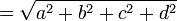
\includegraphics[scale=.6]{graphics/cac27278c238ea97dbd86baa6afd19fe.png}
\item
  The negative of a quaternion:\\\texttt{=(-a, -b, -c, -d)}
\item
  The conjugate of a quaternion:\\\texttt{=( a, -b, -c, -d)}
\item
  Addition of a real number r and a quaternion
  q:\\\texttt{r + q = q + r = (a+r, b, c, d)}
\item
  Addition of two
  quaternions:\\\texttt{q1 + q2 = (a1+a2, b1+b2, c1+c2, d1+d2)}
\item
  Multiplication of a real number and a
  quaternion:\\\texttt{qr = rq = (ar, br, cr, dr)}
\item
  Multiplication of two quaternions q\textsubscript{1} and
  q\textsubscript{2} is given
  by:\\\texttt{( a1a2 − b1b2 − c1c2 − d1d2,}\\\texttt{~ a1b2 + b1a2 + c1d2 − d1c2,}\\\texttt{~ a1c2 − b1d2 + c1a2 + d1b2,}\\\texttt{~ a1d2 + b1c2 − c1b2 + d1a2 )}
\item
  Show that, for the two quaternions q\textsubscript{1} and
  q\textsubscript{2}:\\\texttt{q1q2~!= q2q1}
\end{enumerate}

If your language has built-in support for quaternions then use it.

C.f.

\begin{itemize}
\item
  \emph{Vector products}
\item
  \href{http://www.maths.tcd.ie/pub/HistMath/People/Hamilton/QLetter/QLetter.pdf}{On
  Quaternions}; or on a new System of Imaginaries in Algebra. By Sir
  William Rowan Hamilton LL.D, P.R.I.A., F.R.A.S., Hon. M. R. Soc. Ed.
  and Dub., Hon. or Corr. M. of the Royal or Imperial Academies of St.
  Petersburgh, Berlin, Turin and Paris, Member of the American Academy
  of Arts and Sciences, and of other Scientific Societies at Home and
  Abroad, Andrews' Prof. of Astronomy in the University of Dublin, and
  Royal Astronomer of Ireland.
\end{itemize}


\begin{wideverbatim}

(scl 6)

(def 'quatCopy copy)

(de quatNorm (Q)
   (sqrt (sum * Q Q)) )

(de quatNeg (Q)
   (mapcar - Q) )

(de quatConj (Q)
   (cons (car Q) (mapcar - (cdr Q))) )

(de quatAddR (Q R)
   (cons (+ R (car Q)) (cdr Q)) )

(de quatAdd (Q1 Q2)
   (mapcar + Q1 Q2) )

(de quatMulR (Q R)
   (mapcar */ (mapcar * Q (circ R)) (1.0 .)) )

(de quatMul (Q1 Q2)
   (mapcar
      '((Ops I)
         (sum '((Op R I) (Op (*/ R (get Q2 I) 1.0))) Ops Q1 I) )
      '((+ - - -) (+ + + -) (+ - + +) (+ + - +))
      '((1 2 3 4) (2 1 4 3) (3 4 1 2) (4 3 2 1)) ) )

(de quatFmt (Q)
   (mapcar '((R S) (pack (format R *Scl) S))
      Q
      '(" + " "i + " "j + " "k") ) )


\end{wideverbatim}

\begin{wideverbatim}


Test:

(setq
   Q (1.0 2.0 3.0 4.0)
   Q1 (2.0 3.0 4.0 5.0)
   Q2 (3.0 4.0 5.0 6.0)
   R 7.0 )

(prinl "R  = " (format R *Scl))
(prinl "Q  = " (quatFmt Q))
(prinl "Q1 = " (quatFmt Q1))
(prinl "Q2 = " (quatFmt Q2))
(prinl)
(prinl "norm(Q)  = " (format (quatNorm Q) *Scl))
(prinl "norm(Q1) = " (format (quatNorm Q1) *Scl))
(prinl "norm(Q2) = " (format (quatNorm Q2) *Scl))
(prinl "net(Q)   = " (quatFmt (quatNeg Q)))
(prinl "conj(Q)  = " (quatFmt (quatConj Q)))
(prinl "Q + R    = " (quatFmt (quatAddR Q R)))
(prinl "Q1 + Q2  = " (quatFmt (quatAdd Q1 Q2)))
(prinl "Q * R    = " (quatFmt (quatMulR Q R)))
(prinl "Q1 * Q2  = " (quatFmt (quatMul Q1 Q2)))
(prinl "Q2 * Q1  = " (quatFmt (quatMul Q2 Q1)))
(prinl (if (= (quatMul Q1 Q2) (quatMul Q2 Q1)) "Equal" "Not equal"))

Output:

R  = 7.000000
Q  = 1.000000 + 2.000000i + 3.000000j + 4.000000k
Q1 = 2.000000 + 3.000000i + 4.000000j + 5.000000k
Q2 = 3.000000 + 4.000000i + 5.000000j + 6.000000k

norm(Q)  = 5.477225
norm(Q1) = 7.348469
norm(Q2) = 9.273618
net(Q)   = -1.000000 + -2.000000i + -3.000000j + -4.000000k
conj(Q)  = 1.000000 + -2.000000i + -3.000000j + -4.000000k
Q + R    = 8.000000 + 2.000000i + 3.000000j + 4.000000k
Q1 + Q2  = 5.000000 + 7.000000i + 9.000000j + 11.000000k
Q * R    = 7.000000 + 14.000000i + 21.000000j + 28.000000k
Q1 * Q2  = -56.000000 + 16.000000i + 24.000000j + 26.000000k
Q2 * Q1  = -56.000000 + 18.000000i + 20.000000j + 28.000000k
Not equal

\end{wideverbatim}

\pagebreak{}
\section*{Simple windowed application}

This task asks to create a window with a label that says ``There have
been no clicks yet'' and a button that says ``click me''. Upon clicking
the button with the mouse, the label should change and show the number
of times the button has been clicked.

\begin{wideverbatim}

The standard PicoLisp GUI is HTTP based. Connect your browser to
http://localhost:8080 after starting the following script.

#!/usr/bin/picolisp /usr/lib/picolisp/lib.l

(load "@ext.l" "@lib/http.l" "@lib/xhtml.l" "@lib/form.l")

(zero *Count)

(de start ()
   (app)
   (action
      (html 0 "Clicks" NIL NIL
         (form NIL
            (gui '(+Init +TextField) "There have been no clicks yet")
            (----)
            (gui '(+JS +Button) "click me"
               '(set> (field -1)
                  (pack "Clicked " (inc '*Count) " times") ) ) ) ) ) )

(server 8080 "!start")
(wait)

\end{wideverbatim}

\pagebreak{}
\section*{Simulate input/Keyboard}

Send simulated keystrokes to a GUI window, or terminal. You should
specify whether the target may be externally created (i.e., if the
keystrokes are going to an application other than the application that
is creating them).

\begin{wideverbatim}

PicoLisp comes with a dedicated browser GUI. A library based on web scraping (in
"lib/scrape.l") can be used to drive that GUI under program control. It allows
to read GUI pages, click on HTML links, enter text into forms, and press submit
buttons. In that way one application can control another application.

The documented [http://software-lab.de/doc/app.html#minApp demo application],
which is also available online at [http://7fach.de/8080 app.7fach.de], is used
in the following example. Keyboard input is simulated with the function 'enter'
to fill the login form's name and password fields.

(load "@lib/http.l" "@lib/scrape.l")

# Connect to the demo app at http://7fach.de/8080
(scrape "7fach.de" 80 "8080")

# Log in
(expect "'admin' logged in"
   (enter 3 "admin")       # Enter user name into 3rd field
   (enter 4 "admin")       # Enter password into 4th field
   (press "login") )       # Press the "login" button

(click "Items")         # Open "Items" dialog
(click "Spare Part")    # Click on "Spare Part" article
(prinl (value 8))       # Print the price (12.50)
(click "logout")        # Log out

Output:

12.50

The same example is used in the related task [[Simulate input/Mouse#PicoLisp]].

\end{wideverbatim}

\pagebreak{}
\section*{Simulate input/Mouse}

Simulate the click of a mouse button by the user. Specify if the target
GUI may be externally created.

\begin{wideverbatim}

PicoLisp comes with a dedicated browser GUI. A library based on web scraping (in
"lib/scrape.l") can be used to drive that GUI under program control. It allows
to read GUI pages, click on HTML links, enter text into forms, and press submit
buttons. In that way one application can control another application.

The documented [http://software-lab.de/doc/app.html#minApp demo application],
which is also available online at [http://7fach.de/8080 app.7fach.de], is used
in the following example. Mouse input is simulated with the functions 'click'
(click on a HTML link) and 'press' (press a submit button).

(load "@lib/http.l" "@lib/scrape.l")
 
# Connect to the demo app at http://7fach.de/8080
(scrape "7fach.de" 80 "8080")
 
# Log in
(expect "'admin' logged in"
   (enter 3 "admin")       # Enter user name into 3rd field
   (enter 4 "admin")       # Enter password into 4th field
   (press "login") )       # Press the "login" button
 
(click "Items")         # Open "Items" dialog
(click "Spare Part")    # Click on "Spare Part" article
(prinl (value 8))       # Print the price (12.50)
(click "logout")        # Log out


Output:
12.50

The same example is used in the related task [[Simulate input/Keyboard#PicoLisp]].

\end{wideverbatim}

\pagebreak{}
\section*{Singleton}

A Global Singleton is a class of which only one instance exists within a
program. Any attempt to use non-static members of the class involves
performing operations on this one instance.

\begin{wideverbatim}

As there is no physical difference between classes and objects, we
can use the class symbol itself.

(class +Singleton)

(dm message1> ()
   (prinl "This is method 1 on " This) )

(dm message2> ()
   (prinl "This is method 2 on " This) )

Output:

: (message1> '+Singleton)
This is method 1 on +Singleton
-> +Singleton

: (message2> '+Singleton)
This is method 2 on +Singleton
-> +Singleton

\end{wideverbatim}

\pagebreak{}
\section*{Singly-linked list/Element definition}

Define the data structure for a \emph{singly-linked list} element.
Said element should contain a data member capable of holding a numeric
value, and the link to the next element should be mutable.

\begin{wideverbatim}

In PicoLisp, the singly-linked list is the most important data structure. Many
built-in functions deal with linked lists. A list consists of interconnected
"cells". Cells are also called "cons pairs", because they are constructed with
the function '[http://software-lab.de/doc/refC.html#cons cons]'.

Each cell consists of two parts: A CAR and a CDR. Both may contain (i.e. point
to) arbitrary data (numbers, symbols, other cells, or even to itself). In the
case of a linked list, the CDR points to the rest of the list.

The CAR of a cell can be manipulated with
'[http://software-lab.de/doc/refS.html#set set]'
and the CDR with '[http://software-lab.de/doc/refC.html#con con]'.

\end{wideverbatim}

\pagebreak{}
\section*{Singly-linked list/Element insertion}

Using the link element defined in \emph{Singly-Linked List (element)},
define a method to insert an element into a \emph{singly-linked list}
following a given element.

Using this method, insert an element C into a list comprised of
elements A $->$ B, following element A.

\begin{wideverbatim}

Destructive operation

(de insertAfter (Item Lst New)
   (when (member Item Lst)
      (con @ (cons New (cdr @))) )
   Lst )

Non-destructive operation

(de insertAfter (Item Lst New)
   (if (index Item Lst)
      (conc (cut @ 'Lst) (cons New Lst))
      Lst ) )

Output in both cases:

: (insertAfter 'A '(A B) 'C)
-> (A C B)

: (insertAfter 'A '(X Y Z A B D E) 'C)
-> (X Y Z A C B D E)

\end{wideverbatim}

\pagebreak{}
\section*{Singly-linked list/Traversal}

Traverse from the beginning of a singly-linked list to the end.

\begin{wideverbatim}

We might use map functions

(mapc println '(a "cde" (X Y Z) 999))

or flow control functions

(for X '(a "cde" (X Y Z) 999)
   (println X) )

Output in both cases:

a
"cde"
(X Y Z)
999

\end{wideverbatim}

\pagebreak{}
\section*{Sleep}

Write a program that does the following in this order:

\begin{itemize}
\item
  Input an amount of time to sleep in whatever units are most natural
  for your language (milliseconds, seconds, ticks, etc.). This unit
  should be noted in comments or in a description.
\item
  \emph{Print} ``Sleeping\ldots{}''
\item
  Sleep the main \emph{thread} for the given amount of
  time.
\item
  Print ``Awake!''
\item
  End.
\end{itemize}

\begin{wideverbatim}

(prinl "Sleeping..." )
(wait 2000)                # Wait for 2 seconds
(prinl "Awake!")

As wait will continue executing background events, another possibility (for a
complete stop) is calling some external program like

(prinl "Sleeping..." )
(call 'sleep 2)            # Wait for 2 seconds
(prinl "Awake!")

\end{wideverbatim}

\pagebreak{}
\section*{Sockets}

For this exercise a program is open a socket to localhost on port 256
and send the message ``hello socket world'' before closing the socket.
Catching any exceptions or errors is not required.

\begin{wideverbatim}

(when (connect "localhost" 256)
   (out @ (prinl "hello socket world"))
   (close @) )

\end{wideverbatim}

\pagebreak{}
\section*{Sokoban}

Demonstrate how to find a solution to a given
\href{http://en.wikipedia.org/wiki/Sokoban}{Sokoban} level. For the
purpose of this task (formally, a PSPACE-complete problem) any method
may be used. However a move-optimal or push-optimal (or any other
-optimal) solutions is preferred.

Sokoban levels are usually stored as a character array where

\begin{itemize}
\item
  \emph{space} is an empty square
\item
  \# is a wall
\item
  @ is the player
\item
  \$ is a box
\item
  . is a goal
\item
  + is the player on a goal
\item
  * is a box on a goal
\end{itemize}

Sokoban solutions are usually stored in the LURD format, where lowercase
l, u, r and d represent a move in that (\textbf{l}eft, \textbf{u}p,
\textbf{r}ight, \textbf{d}own) direction and capital LURD represents a
push.

Please state if you use some other format for either the input or
output, and why.

For more information, see
\href{http://www.sokobano.de/wiki/index.php?title=Main\_Page}{the
Sokoban wiki}.

\begin{wideverbatim}

This searches for a solution, without trying for the push-optimal one. The
player moves between the pushes, however, are minimized.

(load "@lib/simul.l")

# Display board
(de display ()
   (disp *Board NIL
      '((This)
         (pack
            (if2 (== This *Pos) (memq This *Goals)
               "+"                   # Player on goal
               "@"                   # Player elsewhere
               (if (: val) "*" ".")  # On gloal
               (or (: val) " ") )    # Elsewhere
            " " ) ) ) )

# Initialize
(de main (Lst)
   (mapc
      '((B L)
         (mapc
            '((This C)
               (case C
                  (" ")
                  ("." (push '*Goals This))
                  ("@" (setq *Pos This))
                  ("\$" (=: val C) (push '*Boxes This))
                  (T (=: val C)) ) )
               B L ) )
      (setq *Board (grid (length (car Lst)) (length Lst)))
      (apply mapcar (flip (mapcar chop Lst)) list) )
   (display) )

# Generate possible push-moves
(de pushes ()
   (make
      (for Box *Boxes
         (unless (or (; (west Box) val) (; (east Box) val))
            (when (moves (east Box))
               (link (cons (cons Box (west Box)) *Pos "L" @)) )
            (when (moves (west Box))
               (link (cons (cons Box (east Box)) *Pos "R" @)) ) )
         (unless (or (; (south Box) val) (; (north Box) val))
            (when (moves (north Box))
               (link (cons (cons Box (south Box)) *Pos "D" @)) )
            (when (moves (south Box))
               (link (cons (cons Box (north Box)) *Pos "U" @)) ) ) ) ) )

\end{wideverbatim}

\begin{wideverbatim}

# Moves of player to destination
(de moves (Dst Hist)
   (or
      (== Dst *Pos)
      (mini length
         (extract
            '((Dir)
               (with ((car Dir) Dst)
                  (cond
                     ((== This *Pos) (cons (cdr Dir)))
                     ((: val))
                     ((memq This Hist))
                     ((moves This (cons Dst Hist))
                        (cons (cdr Dir) @) ) ) ) )
            '((west . "r") (east . "l") (south . "u") (north . "d")) ) ) ) )

# Find solution
(de go (Res)
   (unless (idx '*Hist (sort (copy *Boxes)) T)  # No repeated state
      (if (find '((This) (<> "\$" (: val))) *Goals)
         (pick
            '((Psh)
               (setq  # Move
                  *Pos (caar Psh)
                  *Boxes (cons (cdar Psh) (delq *Pos *Boxes)) )
               (put *Pos 'val NIL)
               (put (cdar Psh) 'val "\$")
               (prog1 (go (append (cddr Psh) Res))
                  (setq  # Undo move
                     *Pos (cadr Psh)
                     *Boxes (cons (caar Psh) (delq (cdar Psh) *Boxes)) )
                  (put (cdar Psh) 'val NIL)
                  (put (caar Psh) 'val "\$") ) )
            (pushes) )
         (display)  # Display solution
         (pack (flip Res)) ) ) )


\end{wideverbatim}

\begin{wideverbatim}


Test:

(main
   (quote
      "#######"
      "#     #"
      "#     #"
      "#. #  #"
      "#. \$\$ #"
      "#.\$\$  #"
      "#.#  @#"
      "#######" ) )
(prinl)
(go)

Output:

 8 # # # # # # #
 7 #           #
 6 #           #
 5 # .   #     #
 4 # .   \$ \$   #
 3 # . \$ \$     #
 2 # . #     @ #
 1 # # # # # # #
   a b c d e f g

 8 # # # # # # #
 7 #           #
 6 # @         #
 5 # *   #     #
 4 # *         #
 3 # *         #
 2 # * #       #
 1 # # # # # # #
   a b c d e f g
-> "uuulDLLulDDurrrrddlUruLLLrrddlUruLdLUUdrruulLulD"

\end{wideverbatim}


\pagebreak{}
\section*{Solve a Hidato puzzle}

The task is to write a program which solves
\href{http://en.wikipedia.org/wiki/Hidato}{Hidato puzzles}.

The rules are:

\begin{itemize}
\item
  You are given a grid with some numbers placed in it. The other squares
  in the grid will be blank.

  \begin{itemize}
  \item
    The grid is not necessarily rectangular.
  \item
    The grid may have holes in it.
  \item
    The grid is always connected.
  \item
    The number ``1'' is always present, as is another number that is
    equal to the number of squares in the grid. Other numbers are
    present so as to force the solution to be unique.
  \item
    It may be assumed that the difference between numbers present on the
    grid is not greater than lucky 13.
  \end{itemize}
\item
  The aim is to place a natural number in each blank square so that in
  the sequence of numbered squares from ``1'' upwards, each square is in
  the \href{http://en.wikipedia.org/wiki/Moore\_neighborhood}{wp:Moore
  neighborhood} of the squares immediately before and after it in the
  sequence (except for the first and last squares, of course, which only
  have one-sided constraints).

  \begin{itemize}
  \item
    Thus, if the grid was overlaid on a chessboard, a king would be able
    to make legal moves along the path from first to last square in
    numerical order.
  \item
    A square may only contain one number.
  \end{itemize}
\item
  In a proper Hidato puzzle, the solution is unique.
\end{itemize}


\pagebreak{}
For example the following problem


\begin{figure}[H]
  \centering
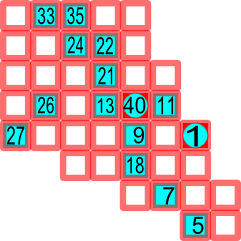
\includegraphics[scale=.9]{graphics/Hidato_Start.png}
\end{figure}


has the following solution, with path marked on it:

\begin{figure}[H]
  \centering
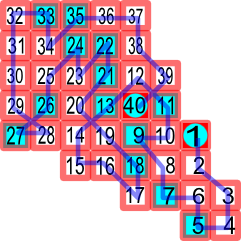
\includegraphics[scale=.9]{graphics/HEnd.png}  
\end{figure}


\begin{wideverbatim}
(load "@lib/simul.l")
 
(de hidato (Lst)
   (let Grid (grid (length (maxi length Lst)) (length Lst))
      (mapc
         '((G L)
            (mapc
               '((This Val)
                  (nond
                     (Val
                        (with (: 0 1 1) (con (: 0 1)))    # Cut off west
                        (with (: 0 1 -1) (set (: 0 1)))   # east
                        (with (: 0 -1 1) (con (: 0 -1)))  # south
                        (with (: 0 -1 -1) (set (: 0 -1))) # north
                        (set This) )
                     ((=T Val) (=: val Val)) ) )
               G L ) )
         Grid
         (apply mapcar (reverse Lst) list) )
      (let Todo
         (by '((This) (: val)) sort
            (mapcan '((Col) (filter '((This) (: val)) Col))
               Grid ) )
         (let N 1
            (with (pop 'Todo)
               (recur (N Todo)
                  (unless (> (inc 'N) (; Todo 1 val))
                     (find
                        '((Dir)
                           (with (Dir This)
                              (cond
                                 ((= N (: val))
                                    (if (cdr Todo) (recurse N @) T) )
                                 ((not (: val))
                                    (=: val N)
                                    (or (recurse N Todo) (=: val NIL)) ) ) ) )
                        (quote
                           west east south north
                           ((X) (or (south (west X)) (west (south X))))
                           ((X) (or (north (west X)) (west (north X))))
                           ((X) (or (south (east X)) (east (south X))))
                           ((X) (or (north (east X)) (east (north X)))) ) ) ) ) ) ) )
      (disp Grid 0
         '((This)
            (if (: val) (align 3 @) "   ") ) ) ) )


\end{wideverbatim}

\begin{wideverbatim}


Test:

(hidato
   (quote
      (T   33  35  T   T)
      (T   T   24  22  T)
      (T   T   T   21  T   T)
      (T   26  T   13  40  11)
      (27  T   T   T   9   T   1)
      (NIL NIL T   T   18  T   T)
      (NIL NIL NIL NIL T   7   T  T)
      (NIL NIL NIL NIL NIL NIL 5  T) ) )

Output:

   +---+---+---+---+---+---+---+---+
 8 | 32  33  35  36  37|   |   |   |
   +   +   +   +   +   +---+---+---+
 7 | 31  34  24  22  38|   |   |   |
   +   +   +   +   +   +---+---+---+
 6 | 30  25  23  21  12  39|   |   |
   +   +   +   +   +   +   +---+---+
 5 | 29  26  20  13  40  11|   |   |
   +   +   +   +   +   +   +---+---+
 4 | 27  28  14  19   9  10   1|   |
   +---+---+   +   +   +   +   +---+
 3 |   |   | 15  16  18   8   2|   |
   +---+---+---+---+   +   +   +---+
 2 |   |   |   |   | 17   7   6   3|
   +---+---+---+---+---+---+   +   +
 1 |   |   |   |   |   |   |  5   4|
   +---+---+---+---+---+---+---+---+
     a   b   c   d   e   f   g   h

\end{wideverbatim}

\pagebreak{}
\section*{Sort an array of composite structures}

Sort an array of composite structures by a key. For example, if you
define a composite structure that presents a name-value pair (in
pseudocode):

\begin{verbatim}
Define structure pair such that: 
   name as a string
   value as a string
\end{verbatim}

and an array of such pairs:

\begin{verbatim}
x: array of pairs
\end{verbatim}

then define a sort routine that sorts the array \emph{x} by the key
\emph{name}.

This task can always be accomplished with \emph{Sorting Using a Custom
  Comparator}. If your language is not listed here, please see the
other article.

\begin{wideverbatim}

By default, the [http://software-lab.de/doc/refS.html#sort sort] function in
PicoLisp returns an ascending list (of any type)

: (sort '(("def" 456) ("abc" 789) ("ghi" 123)))
-> (("abc" 789) ("def" 456) ("ghi" 123))

To sort by a certain sub-element, the function
[http://software-lab.de/doc/refB.html#by by] can be used. For example, to
sort by the first element

: (by car sort '(("def" 456) ("abc" 789) ("ghi" 123)))
-> (("abc" 789) ("def" 456) ("ghi" 123))

or by the second element

: (by cadr sort '(("def" 456) ("abc" 789) ("ghi" 123)))
-> (("ghi" 123) ("def" 456) ("abc" 789))

\end{wideverbatim}

\pagebreak{}
\section*{Sort an integer array}

Sort an array (or list) of integers in ascending numerical order. Use a
sorting facility provided by the language/library if possible.

\begin{wideverbatim}

The [http://software-lab.de/doc/refS.html#sort sort] function in
PicoLisp returns already by default an ascending list (of any type,
not only integers):

(sort (2 4 3 1 2))
-> (1 2 2 3 4)

\end{wideverbatim}

\pagebreak{}
\section*{Sort disjoint sublist}

Given a list of values and a set of integer indices into that value
list, the task is to sort the values at the given indices, but
preserving the values at indices outside the set of those to be sorted.

Make your example work with the following list of values and set of
indices: \texttt{ }

\begin{verbatim}
   values: [7, 6, 5, 4, 3, 2, 1, 0]
   indices: {6, 1, 7}
\end{verbatim}

Where the correct result would be:

\begin{verbatim}
   [7, 0, 5, 4, 3, 2, 1, 6].
\end{verbatim}

Note that for one based, rather than the zero-based indexing above, use
the \texttt{indices: \{7, 2, 8\}}. The indices are described as a set
rather than a list but any collection-type of those indices without
duplication may be used as long as the example is insensitive to the
order of indices given.

\begin{wideverbatim}

The indices are incremented here, as PicoLisp is 1-based

(let (Values (7 6 5 4 3 2 1 0)  Indices (7 2 8))
   (mapc
      '((V I) (set (nth Values I) V))
      (sort (mapcar '((N) (get Values N)) Indices))
      (sort Indices) )
   Values )

Output:

-> (7 0 5 4 3 2 1 6)

\end{wideverbatim}

\pagebreak{}
\section*{Sort stability}

When sorting records in a table by a particular column or field, a
\href{http://en.wikipedia.org/wiki/Stable\_sort\#Stability}{stable sort}
will always retain the relative order of records that have the same key.

For example, in this table of countries and cities, a stable sort on the
\textbf{second} column, the cities, would keep the US Birmingham above
the UK Birmingham. (Although an unstable sort \emph{might}, in this
case, place the US Birmingham above the UK Birmingham, a stable sort
routine would \emph{guarantee} it).

\begin{verbatim}
UK  London
US  New York
US  Birmingham
UK  Birmingham
\end{verbatim}

Similarly, stable sorting on just the first column would generate ``UK
London'' as the first item and ``US Birmingham'' as the last item (since
the order of the elements having the same first word -- ``UK'' or ``US''
-- would be maintained).

\begin{enumerate}
\item
  Examine the documentation on any in-built sort routines supplied by a
  language.
\item
  Indicate if an in-built routine is supplied
\item
  If supplied, indicate whether or not the in-built routine is stable.
\end{enumerate}

(This
\href{http://en.wikipedia.org/wiki/Stable\_sort\#Comparison\_of\_algorithms}{Wikipedia
table} shows the stability of some common sort routines).


\begin{wideverbatim}

The [http://software-lab.de/doc/refS.html#sort sort] function is unstable

\end{wideverbatim}

\pagebreak{}
\section*{Sort using a custom comparator}

Sort an array (or list) of strings in order of descending length, and in
ascending lexicographic order for strings of equal length. Use a sorting
facility provided by the language/library, combined with your own
callback comparison function.

\textbf{Note:} Lexicographic order is case-insensitive.

\begin{wideverbatim}

By default, the [http://software-lab.de/doc/refS.html#sort sort] function in
PicoLisp returns an ascending list (of any type). To get a result in descending
order, the "greater than" function can be supplied

: (sort '("def" "abc" "ghi") >)
-> ("ghi" "def" "abc")

or simply the result reversed (which is, btw, the most efficient way)

: (flip (sort '("def" "abc" "ghi")))
-> ("ghi" "def" "abc")

\end{wideverbatim}

\pagebreak{}
\section*{Sorting algorithms/Bead sort}

\textbf{Sorting Algorithm}\\ This is a sorting algorithm. It may be
applied to a set of data in order to sort it.

For other sorting algorithms, see
\emph{Category:Sorting Algorithms},
or:

\textbf{\emph{O}(\emph{n} log\emph{n})
Sorts}\\\emph{Heapsort} \textbar{}
\emph{Mergesort} \textbar{}
\emph{Quicksort}\\\textbf{\emph{O}(\emph{n}
log\textsuperscript{2}\emph{n})
Sorts}\\\emph{Shell~Sort}\\\textbf{\emph{O}(\emph{n}\textsuperscript{2})
Sorts}\\\emph{Bubble~sort}
\textbar{}
\emph{Cocktail~sort}
\textbar{} \emph{Comb~sort}
\textbar{} \emph{Gnome~sort}
\textbar{}
\emph{Insertion~sort}
\textbar{}
\emph{Selection~sort}
\textbar{} \emph{Strand~sort}
\\\textbf{Other Sorts}\\\textbf{Bead~sort} \textbar{}
\emph{Bogosort} \textbar{}
\emph{Counting~sort}
\textbar{} \emph{Pancake~sort}
\textbar{}
\emph{Permutation~sort}
\textbar{} \emph{Radix~sort}
\textbar{} \emph{Sleep~sort}
\textbar{} \emph{Stooge~sort}

In this task, the goal is to sort an array of positive integers using
the \href{http://en.wikipedia.org/wiki/Bead\_sort}{Bead Sort Algorithm}.

Algorithm has O(S), where S is the sum of the integers in the input set:
Each bead is moved individually. This is the case when bead sort is
implemented without a mechanism to assist in finding empty spaces below
the beads, such as in software implementations.


\begin{wideverbatim}

The following implements a direct model of the bead sort algorithm.
Each pole is a list of 'T' symbols for the beads.

(de beadSort (Lst)
   (let Abacus (cons NIL)
      (for N Lst                                   # Thread beads on poles
         (for (L Abacus  (ge0 (dec 'N))  (cdr L))
            (or (cdr L) (queue 'L (cons)))
            (push (cadr L) T) ) )
      (make
         (while (gt0 (cnt pop (cdr Abacus)))       # Drop and count beads
            (link @) ) ) ) )

Output:

: (beadSort (5 3 1 7 4 1 1 20))
-> (20 7 5 4 3 1 1 1)

\end{wideverbatim}

\pagebreak{}
\section*{Sorting algorithms/Bogosort}

\href{http://en.wikipedia.org/wiki/Bogosort}{Bogosort} a list of
numbers. Bogosort simply shuffles a collection randomly until it is
sorted.

``Bogosort'' is a perversely inefficient algorithm only used as an
in-joke. Its average run-time is O(n!) because the chance that any given
shuffle of a set will end up in sorted order is about one in \emph{n}
factorial, and the worst case is infinite since there's no guarantee
that a random shuffling will ever produce a sorted sequence. Its best
case is O(n) since a single pass through the elements may suffice to
order them.

Pseudocode:

\begin{verbatim}
while not InOrder(list) do
   Shuffle(list)
done
\end{verbatim}

The \emph{Knuth shuffle} may be used to implement
the shuffle part of this algorithm.

\begin{wideverbatim}

(de bogosort (Lst)
   (loop
      (map
         '((L) (rot L (rand 1 (length L))))
         Lst )
      (T (apply <= Lst) Lst) ) )

Output:

: (bogosort (make (do 9 (link (rand 1 999)))))
-> (1 167 183 282 524 556 638 891 902)

: (bogosort (make (do 9 (link (rand 1 999)))))
-> (20 51 117 229 671 848 883 948 978)

: (bogosort (make (do 9 (link (rand 1 999)))))
-> (1 21 72 263 391 476 794 840 878)

\end{wideverbatim}

\pagebreak{}
\section*{Sorting algorithms/Bubble sort}

In this task, the goal is to sort an array of elements using the bubble
sort algorithm. The elements must have a total order and the index of
the array can be of any discrete type. For languages where this is not
possible, sort an array of integers.

The bubble sort is generally considered to be the simplest sorting
algorithm. Because of its simplicity and ease of visualization, it is
often taught in introductory computer science courses. Because of its
abysmal O(n\textsuperscript{2}) performance, it is not used often for
large (or even medium-sized) datasets.

The bubble sort works by passing sequentially over a list, comparing
each value to the one immediately after it. If the first value is
greater than the second, their positions are switched. Over a number of
passes, at most equal to the number of elements in the list, all of the
values drift into their correct positions (large values ``bubble''
rapidly toward the end, pushing others down around them). Because each
pass finds the maximum item and puts it at the end, the portion of the
list to be sorted can be reduced at each pass. A boolean variable is
used to track whether any changes have been made in the current pass;
when a pass completes without changing anything, the algorithm exits.

This can be expressed in pseudocode as follows (assuming 1-based
indexing):

\begin{wideverbatim}
repeat
    hasChanged := false
    decrement itemCount
    repeat with index from 1 to itemCount
        if (item at index) > (item at (index + 1))
            swap (item at index) with (item at (index + 1))
            hasChanged := true
until hasChanged = false
\end{wideverbatim}

\begin{description}
\item[References]
\end{description}

\begin{itemize}
\item
  The article on
  \href{http://en.wikipedia.org/wiki/Bubble\_sort}{Wikipedia}.
\item
  Dance
  \href{http://www.youtube.com/watch?v=lyZQPjUT5B4\&feature=youtu.be}{interpretation}.
\{itemize}


\begin{wideverbatim}

(de bubbleSort (Lst)
   (use Chg
      (loop
         (off Chg)
         (for (L Lst (cdr L) (cdr L))
            (when (> (car L) (cadr L))
               (xchg L (cdr L))
               (on Chg) ) )
         (NIL Chg Lst) ) ) )

\end{wideverbatim}

\pagebreak{}
\section*{Sorting algorithms/Cocktail sort}

The cocktail shaker sort is an improvement on the \emph{Bubble Sort}.
The improvement is basically that values ``bubble'' both directions
through the array, because on each iteration the cocktail shaker sort
bubble sorts once forwards and once backwards. Pseudocode for the
algorithm (from
\href{http://en.wikipedia.org/wiki/Cocktail\_sort}{wikipedia}):

\begin{wideverbatim}
function cocktailSort( A : list of sortable items )
 do
   swapped := false
   for each i in 0 to length( A ) - 2 do
     if A[ i ] > A[ i+1 ] then // test whether the two 
                               // elements are in the wrong 
                               // order
       swap( A[ i ], A[ i+1 ] ) // let the two elements
                                // change places
       swapped := true;
   if swapped = false then
     // we can exit the outer loop here if no swaps occurred.
     break do-while loop;
   swapped := false
   for each i in length( A ) - 2 down to 0 do
     if A[ i ] > A[ i+1 ] then
       swap( A[ i ], A[ i+1 ] )
       swapped := true;
 while swapped; // if no elements have been swapped, 
                // then the list is sorted
\end{wideverbatim}



\begin{wideverbatim}

(de cocktailSort (Lst)
   (use (Swapped L)
      (loop
         (off Swapped)
         (setq L Lst)
         (while (cdr L)
            (when (> (car L) (cadr L))
               (xchg L (cdr L))
               (on Swapped) )
            (pop 'L) )
         (NIL Swapped Lst)
         (off Swapped)
         (loop
            (setq L (prior L Lst))  # Not recommended (inefficient)
            (when (> (car L) (cadr L))
               (xchg L (cdr L))
               (on Swapped) )
            (T (== Lst L)) )
         (NIL Swapped Lst) ) ) )

Output:

: (cocktailSort (make (do 9 (link (rand 1 999)))))
-> (1 167 183 282 524 556 638 891 902)
: (cocktailSort (make (do 9 (link (rand 1 999)))))
-> (82 120 160 168 205 226 408 708 719)

\end{wideverbatim}

\pagebreak{}
\section*{Sorting algorithms/Comb sort}

The \textbf{Comb Sort} is a variant of the \emph{Bubble Sort}. Like
the \emph{Shell sort}, the Comb Sort increases the gap used in
comparisons and exchanges (dividing the gap by
\includegraphics[scale=.6][scale=.6]{graphics/84f07409bec0076ebf75277eeffbd5c4.png}
works best, but 1.3 may be more practical). Some implementations use the
insertion sort once the gap is less than a certain amount. See the
\href{http://en.wikipedia.org/wiki/Comb\_sort}{article on Wikipedia}.
Variants:

\begin{itemize}
\item
  Combsort11 makes sure the gap ends in (11, 8, 6, 4, 3, 2, 1), which is
  significantly faster than the other two possible endings
\item
  Combsort with different endings changes to a more efficient sort when
  the data is almost sorted (when the gap is small). Comb sort with a
  low gap isn't much better than the Bubble Sort.
\end{itemize}

Pseudocode:

\begin{wideverbatim}
function combsort(array input)
    gap := input.size //initialize gap size
    loop until gap = 1 and swaps = 0
        //update the gap value for a next comb. Below is an example
        gap := int(gap / 1.25)
        if gap < 1
          //minimum gap is 1
          gap := 1
        end if
        i := 0
        swaps := 0 //see Bubble Sort for an explanation
        //a single "comb" over the input list
        loop until i + gap >= input.size //see Shell sort for similar idea
            if input[i] > input[i+gap]
                swap(input[i], input[i+gap])
                swaps := 1 // Flag a swap has occurred, so the
                           // list is not guaranteed sorted
            end if
            i := i + 1
        end loop
    end loop
end function
\end{wideverbatim}



\begin{wideverbatim}

(de combSort (Lst)
   (let (Gap (length Lst)  Swaps NIL)
      (while (or (> Gap 1) Swaps)
         (setq Gap (max 1 (/ (* Gap 4) 5)))
         (off Swaps)
         (use Lst
            (for (G (cdr (nth Lst Gap))  G  (cdr G))
               (when (> (car Lst) (car G))
                  (xchg Lst G)
                  (on Swaps) )
               (pop 'Lst) ) ) ) )
   Lst )

Output:

: (combSort (88 18 31 44 4 0 8 81 14 78 20 76 84 33 73 75 82 5 62 70))
-> (0 4 5 8 14 18 20 31 33 44 62 70 73 75 76 78 81 82 84 88)

\end{wideverbatim}

\pagebreak{}
\section*{Sorting algorithms/Counting sort}

Implement the
\href{http://en.wikipedia.org/wiki/Counting\_sort}{Counting sort}.
This is a way of sorting integers when the minimum and maximum value
are known.

Pseudocode:

\begin{wideverbatim}
function countingSort(array, min, max):
    count: array of (max - min + 1) elements
    initialize count with 0
    for each number in array do
        count[number - min] := count[number - min] + 1
    done
    z := 0
    for i from min to max do
        while ( count[i - min] > 0 ) do
            array[z] := i
            z := z+1
            count[i - min] := count[i - min] - 1
        done
    done
\end{wideverbatim}

The \emph{min} and \emph{max} can be computed apart, or be known \emph{a
priori}.

\textbf{Note}: we know that, given an array of integers, its maximum and
minimum values can be always found; but if we imagine the worst case for
an array of 32 bit integers, we see that in order to hold the counts, we
need an array of 2\textsuperscript{32} elements, i.e., we need, to hold
a count value up to 2\textsuperscript{32}-1, more or less 4 Gbytes. So
the counting sort is more practical when the range is (very) limited and
minimum and maximum values are known \emph{a priori}. (Anyway sparse
arrays may limit the impact of the memory usage)


\begin{wideverbatim}

(de countingSort (Lst Min Max)
   (let Count (need (- Max Min -1) 0)
      (for N Lst
         (inc (nth Count (- N Min -1))) )
      (make
         (map
            '((C I)
               (do (car C) (link (car I))) )
            Count
            (range Min Max) ) ) ) )

Output:

: (countingSort (5 3 1 7 4 1 1 20) 1 20)
-> (1 1 1 3 4 5 7 20)

\end{wideverbatim}

\pagebreak{}
\section*{Sorting algorithms/Gnome sort}

Gnome sort is a sorting algorithm which is similar to \emph{Insertion
  sort}, except that moving an element to its proper place is
accomplished by a series of swaps, as in \emph{Bubble Sort}.

The pseudocode for the algorithm is:

\begin{wideverbatim}
function gnomeSort(a[0..size-1])
    i := 1
    j := 2
    while i < size do
        if a[i-1] <= a[i] then
            // for descending sort, use >= for comparison
            i := j
            j := j + 1 
        else
            swap a[i-1] and a[i]
            i := i - 1
            if i = 0 then
                i := j
                j := j + 1
            endif
        endif
    done
\end{wideverbatim}

\textbf{Task}: implement the Gnome sort in your language to sort an
array (or list) of numbers.

\begin{wideverbatim}
(de gnomeSort (Lst)
   (let J (cdr Lst)
      (for (I Lst (cdr I))
         (if (>= (cadr I) (car I))
            (setq I J  J (cdr J))
            (xchg I (cdr I))
            (if (== I Lst)
               (setq I J  J (cdr J))
               (setq I (prior I Lst)) ) ) ) )
   Lst )

\end{wideverbatim}

\pagebreak{}
\section*{Sorting algorithms/Heapsort}

\href{http://en.wikipedia.org/wiki/Heapsort}{Heapsort} is an in-place
sorting algorithm with worst case and average complexity of
O(\emph{n} log\emph{n}). The basic idea is to turn the array into a
binary heap structure, which has the property that it allows efficient
retrieval and removal of the maximal element. We repeatedly ``remove''
the maximal element from the heap, thus building the sorted list from
back to front. Heapsort requires random access, so can only be used on
an array-like data structure.

Pseudocode:

\begin{wideverbatim}
function heapSort(a, count) is
   input: an unordered array a of length count
 
   (first place a in max-heap order)
   heapify(a, count)
 
   end := count - 1
   while end > 0 do
      (swap the root(maximum value) of the heap with the
       last element of the heap)
      swap(a[end], a[0])
      (decrement the size of the heap so that the previous
       max value will stay in its proper place)
      end := end - 1
      (put the heap back in max-heap order)
      siftDown(a, 0, end)
\end{wideverbatim}

\begin{wideverbatim}
function heapify(a,count) is
   (start is assigned the index in a of the last parent node)
   start := (count - 2) / 2
   
   while start ≥ 0 do
      (sift down the node at index start to the proper place
       such that all nodes below the start index are in heap
       order)
      siftDown(a, start, count-1)
      start := start - 1
   (after sifting down the root all nodes/elements are in heap order)
 
function siftDown(a, start, end) is
   (end represents the limit of how far down the heap to sift)
   root := start

   while root * 2 + 1 ≤ end do       (While the root has at least one child)
      child := root * 2 + 1           (root*2+1 points to the left child)
      (If the child has a sibling and the child's value is less than its sibling's...)
      if child + 1 ≤ end and a[child] < a[child + 1] then
         child := child + 1           (... then point to the right child instead)
      if a[root] < a[child] then     (out of max-heap order)
         swap(a[root], a[child])
         root := child                (repeat to continue sifting down the child now)
      else
         return
\end{wideverbatim}

Write a function to sort a collection of integers using heapsort.

\begin{wideverbatim}

(de heapSort (A Cnt)
   (let Cnt (length A)
      (for (Start (/ Cnt 2) (gt0 Start) (dec Start))
         (siftDown A Start (inc Cnt)) )
      (for (End Cnt (> End 1) (dec End))
         (xchg (nth A End) A)
         (siftDown A 1 End) ) )
   A )

(de siftDown (A Start End)
   (use Child
      (for (Root Start  (> End (setq Child (* 2 Root))))
         (and
            (> End (inc Child))
            (> (get A (inc Child)) (get A Child))
            (inc 'Child) )
         (NIL (> (get A Child) (get A Root)))
         (xchg (nth A Root) (nth A Child))
         (setq Root Child) ) ) )

Output:

: (heapSort (make (do 9 (link (rand 1 999)))))
-> (1 167 183 282 524 556 638 891 902)

\end{wideverbatim}

\pagebreak{}
\section*{Sorting algorithms/Insertion sort}

An \emph{O}(\emph{n}\textsuperscript{2}) sorting algorithm
which moves elements one at a time into the correct position. The
algorithm consists of inserting one element at a time into the
previously sorted part of the array, moving higher ranked elements up as
necessary. To start off, the first (or smallest, or any arbitrary)
element of the unsorted array is considered to be the sorted part.

Although insertion sort is an \emph{O}(\emph{n}\textsuperscript{2})
algorithm, its simplicity, low overhead, good locality of reference
and efficiency make it a good choice in two cases (i) small \emph{n},
(ii) as the final finishing-off algorithm for \emph{O}(\emph{n}
log\emph{n}) algorithms such as \emph{mergesort} and \emph{quicksort}.

The algorithm is as follows (from
\href{http://en.wikipedia.org/wiki/Insertion\_sort\#Algorithm}{wikipedia}):

\begin{wideverbatim}
function insertionSort(array A)
    for i from 1 to length[A]-1 do
        value := A[i] 
        j := i-1
        while j >= 0 and A[j] > value do
            A[j+1] := A[j]
            j := j-1
        done
        A[j+1] = value
    done
\end{wideverbatim}

Writing the algorithm for integers will suffice.

\begin{wideverbatim}

(de insertionSort (Lst)
   (for (I (cdr Lst)  I  (cdr I))
      (for (J Lst  (n== J I)  (cdr J))
         (T (> (car J) (car I))
            (rot J (offset I J)) ) ) )
   Lst )

Output:

: (insertionSort (5 3 1 7 4 1 1 20))
-> (1 1 1 3 4 5 7 20)

\end{wideverbatim}

% \pagebreak{}
% \section*{Sorting algorithms/Merge sort}


% The \textbf{merge sort} is a recursive sort of order n*log(n). It is
% notable for having a worst case and average complexity of
% \emph{O(n*log(n))}, and a best case complexity of \emph{O(n)} (for
% pre-sorted input). The basic idea is to split the collection into
% smaller groups by halving it until the groups only have one element or
% no elements (which are both entirely sorted groups). Then merge the
% groups back together so that their elements are in order. This is how
% the algorithm gets its ``divide and conquer'' description.

% Write a function to sort a collection of integers using the merge sort.
% The merge sort algorithm comes in two parts: a sort function and a merge
% function. The functions in pseudocode look like this:

% \begin{verbatim}
% function mergesort(m)
%    var list left, right, result
%    if length(m) ≤ 1
%        return m
%    else
%        var middle = length(m) / 2
%        for each x in m up to middle - 1
%            add x to left
%        for each x in m at and after middle
%            add x to right
%        left = mergesort(left)
%        right = mergesort(right)
%        if last(left) ≤ first(right) 
%           append right to left
%           return left
%        result = merge(left, right)
%        return result

% function merge(left,right)
%    var list result
%    while length(left) > 0 and length(right) > 0
%        if first(left) ≤ first(right)
%            append first(left) to result
%            left = rest(left)
%        else
%            append first(right) to result
%            right = rest(right)
%    if length(left) > 0 
%        append rest(left) to result
%    if length(right) > 0 
%        append rest(right) to result
%    return result
% \end{verbatim}

% For more information see
% \href{http://en.wikipedia.org/wiki/Merge\_sort}{Wikipedia}



% \begin{wideverbatim}

% {IanOsgood}

% \end{wideverbatim}

\pagebreak{}
\section*{Sorting algorithms/Pancake sort}

Sort an array of integers (of any convenient size) into ascending order
using \href{http://en.wikipedia.org/wiki/Pancake\_sorting}{Pancake
sorting}. In short, instead of individual elements being sorted, the
only operation allowed is to ``flip'' one end of the list, like so:

\begin{verbatim}
Before:
6 7 8 9 2 5 3 4 1
After:
9 8 7 6 2 5 3 4 1
\end{verbatim}

Only one end of the list can be flipped; this should be the low end, but
the high end is okay if it's easier to code or works better, but it
\textbf{must} be the same end for the entire solution. (The end flipped
can't be arbitrarily changed.)

Show both the initial, unsorted list and the final sorted list.
(Intermediate steps during sorting are optional.) Optimizations are
optional (but recommended).

For more information on pancake sorting, see
\href{http://en.wikipedia.org/wiki/Pancake\_sorting}{the Wikipedia
entry}.

See also: \emph{Number reversal game}


\begin{wideverbatim}

(de pancake (Lst)
   (prog1 (flip Lst (index (apply max Lst) Lst))
      (for (L @  (cdr (setq Lst (cdr L)))  (cdr L))
         (con L (flip Lst (index (apply max Lst) Lst))) ) ) )

Output:

: (trace 'flip)
-> flip

: (pancake (6 7 2 1 8 9 5 3 4))
 flip : (6 7 2 1 8 9 5 3 4) 6
 flip = (9 8 1 2 7 6 5 3 4)
 flip : (8 1 2 7 6 5 3 4) 1
 flip = (8 1 2 7 6 5 3 4)
 flip : (1 2 7 6 5 3 4) 3
 flip = (7 2 1 6 5 3 4)
 flip : (2 1 6 5 3 4) 3
 flip = (6 1 2 5 3 4)
 flip : (1 2 5 3 4) 3
 flip = (5 2 1 3 4)
 flip : (2 1 3 4) 4
 flip = (4 3 1 2)
 flip : (3 1 2) 1
 flip = (3 1 2)
 flip : (1 2) 2
 flip = (2 1)
-> (9 8 7 6 5 4 3 2 1)

\end{wideverbatim}

\pagebreak{}
\section*{Sorting algorithms/Permutation sort}

Permutation sort, which proceeds by generating the possible permutations
of the input array/list until discovering the sorted one.

Pseudocode:

\begin{verbatim}
while not InOrder(list) do
    nextPermutation(list)
done
\end{verbatim}



\begin{wideverbatim}

(de permutationSort (Lst)
   (let L Lst
      (recur (L)  # Permute
         (if (cdr L)
            (do (length L)
               (T (recurse (cdr L)) Lst)
               (rot L)
               NIL )
            (apply <= Lst) ) ) ) )

Output:

: (permutationSort (make (do 9 (link (rand 1 999)))))
-> (82 120 160 168 205 226 408 708 719)

: (permutationSort (make (do 9 (link (rand 1 999)))))
-> (108 212 330 471 667 716 739 769 938)

: (permutationSort (make (do 9 (link (rand 1 999)))))
-> (118 253 355 395 429 548 890 900 983)

\end{wideverbatim}

% \pagebreak{}
% \section*{Sorting algorithms/Quicksort}

% The task is to sort an array (or list) elements using the
% \emph{quicksort} algorithm. The elements must have a strict weak order
% and the index of the array can be of any discrete type. For languages
% where this is not possible, sort an array of integers.

% Quicksort, also known as \emph{partition-exchange sort}, uses these
% steps.

% \begin{enumerate}
% \item
%   Choose any element of the array to be the pivot.
% \item
%   Divide all other elements (except the pivot) into two partitions.

%   \begin{itemize}
%   \item
%     All elements less than the pivot must be in the first partition.
%   \item
%     All elements greater than the pivot must be in the second partition.
%   \end{itemize}
% \item
%   Use recursion to sort both partitions.
% \item
%   Join the first sorted partition, the pivot, and the second sorted
%   partition.
% \end{enumerate}

% The best pivot creates partitions of equal length (or lengths differing
% by 1). The worst pivot creates an empty partition (for example, if the
% pivot is the first or last element of a sorted array). The runtime of
% Quicksort ranges from \emph{\emph{O}(n}log\emph{n)} with the
% best pivots, to \emph{\emph{O}(n\textsuperscript{2})} with the
% worst pivots, where \emph{n} is the number of elements in the array.

% This is a simple quicksort algorithm, adapted from Wikipedia.

% \begin{wideverbatim}
% function quicksort(array)
%     less, equal, greater := three empty arrays
%     if length(array) > 1  
%         pivot := select any element of array
%         for each x in array
%             if x < pivot then add x to less
%             if x = pivot then add x to equal
%             if x > pivot then add x to greater
%         quicksort(less)
%         quicksort(greater)
%         array := concatenate(less, equal, greater)
% \end{wideverbatim}

% A better quicksort algorithm works in place, by swapping elements within
% the array, to avoid the memory allocation of more arrays.

% \begin{wideverbatim}
% function quicksort(array)
%     if length(array) > 1
%         pivot := select any element of array
%         left := first index of array
%         right := last index of array
%         while left ≤ right
%             while array[left] < pivot
%                 left := left + 1
%             while array[right] > pivot
%                 right := right - 1
%             if left ≤ right
%                 swap array[left] with array[right]
%                 left := left + 1
%                 right := right - 1
%         quicksort(array from first index to right)
%         quicksort(array from left to last index)
% \end{wideverbatim}

% Quicksort has a reputation as the fastest sort. Optimized variants of
% quicksort are common features of many languages and libraries. One often
% contrasts quicksort with
% \emph{merge sort}, because both
% sorts have an average time of \emph{\emph{O}(n}log\emph{n)}.

% \emph{``On average, mergesort does fewer comparisons than quicksort, so
% it may be better when complicated comparison routines are used.
% Mergesort also takes advantage of pre-existing order, so it would be
% favored for using sort() to merge several sorted arrays. On the other
% hand, quicksort is often faster for small arrays, and on arrays of a few
% distinct values, repeated many times.''} ---
% \href{http://perldoc.perl.org/sort.html}{http://perldoc.perl.org/sort.html}

% Quicksort is at one end of the spectrum of divide-and-conquer
% algorithms, with merge sort at the opposite end.

% \begin{itemize}
% \item
%   Quicksort is a conquer-then-divide algorithm, which does most of the
%   work during the partitioning and the recursive calls. The subsequent
%   reassembly of the sorted partitions involves trivial effort.
% \item
%   Merge sort is a divide-then-conquer algorithm. The partioning happens
%   in a trivial way, by splitting the input array in half. Most of the
%   work happens during the recursive calls and the merge phase.
% \end{itemize}

% With quicksort, every element in the first partition is less than or
% equal to every element in the second partition. Therefore, the merge
% phase of quicksort is so trivial that it needs no mention!

% This task has not specified whether to allocate new arrays, or sort in
% place. This task also has not specified how to choose the pivot element.
% (Common ways to are to choose the first element, the middle element, or
% the median of three elements.) Thus there is a variety among the
% following implementations.

% \begin{wideverbatim}

% {IanOsgood}

% \end{wideverbatim}

\pagebreak{}
\section*{Sorting algorithms/Radix sort}

In this task, the goal is to sort an integer array with the
\href{http://en.wikipedia.org/wiki/Radix\_sort}{radix sort algorithm}.
The primary purpose is to complete the characterization of sort
algorithms task.

\begin{wideverbatim}

This is a LSD base-2 radix sort using queues:

(de radixSort (Lst)
   (let Mask 1
      (while
         (let (Pos (list NIL NIL)  Neg (list NIL NIL)  Flg)
            (for N Lst
               (queue
                  (if2 (ge0 N) (bit? Mask N)
                     (cdr Pos) Pos Neg (cdr Neg) )
                  N )
               (and (>= (abs N) Mask) (on Flg)) )
            (setq
               Lst (conc (apply conc Neg) (apply conc Pos))
               Mask (* 2 Mask) )
            Flg ) ) )
   Lst )

Output:

: (radixSort (make (do 12 (link (rand -999 999)))))
-> (-999 -930 -666 -336 -218 68 79 187 391 405 697 922)

\end{wideverbatim}

\pagebreak{}
\section*{Sorting algorithms/Selection sort}

In this task, the goal is to sort an \emph{array} (or list)
of elements using the Selection sort algorithm. It works as follows:

First find the smallest element in the array and exchange it with the
element in the first position, then find the second smallest element and
exchange it with the element in the second position, and continue in
this way until the entire array is sorted. Its asymptotic complexity is
\emph{O}(n\textsuperscript{2}) making it inefficient on large
arrays. Its primary purpose is for when writing data is very expensive
(slow) when compared to reading, eg writing to flash memory or EEPROM.
No other sorting algorithm has less data movement.

For more information see the article on
\href{http://en.wikipedia.org/wiki/Selection\_sort}{Wikipedia}.

\begin{wideverbatim}

(de selectionSort (Lst)
   (map
      '((L) (and (cdr L) (xchg L (member (apply min @) L))))
      Lst )
   Lst )

\end{wideverbatim}

\pagebreak{}
\section*{Sorting algorithms/Shell sort}

In this task, the goal is to sort an array of elements using the
\href{http://en.wikipedia.org/wiki/Shell\_sort}{Shell sort} algorithm, a
diminishing increment sort. The Shell sort is named after its inventor,
Donald Shell, who published the algorithm in 1959. Shellsort is a
sequence of interleaved insertion sorts based on an increment sequence.
The increment size is reduced after each pass until the increment size
is 1. With an increment size of 1, the sort is a basic insertion sort,
but by this time the data is guaranteed to be almost sorted, which is
insertion sort's ``best case''. Any sequence will sort the data as long
as it ends in 1, but some work better than others. Empirical studies
have shown a geometric increment sequence with a ratio of about 2.2 work
well in practice. \href{http://www.cs.princeton.edu/~rs/shell/}{{[}1{]}}
Other good sequences are found at the
\href{https://oeis.org/search?q=shell+sort}{On-Line Encyclopedia of
Integer Sequences}.

\begin{wideverbatim}

(de shellSort (A)
   (for (Inc (*/ (length A) 2)  (gt0 Inc)  (*/ Inc 10 22))
      (for (I Inc  (get A I)  (inc I))
         (let (Tmp @  J I)
            (while (and (>= J Inc) (> (get A (- J Inc)) Tmp))
               (set (nth A J) (get A (- J Inc)))
               (dec 'J Inc) )
            (set (nth A J) Tmp) ) ) )
   A )

Output:

: (shellSort (make (do 9 (link (rand 1 999)))))
-> (1 167 183 282 524 556 638 891 902)

: (shellSort (make (do 9 (link (rand 1 999)))))
-> (82 120 160 168 205 226 408 708 719)

: (shellSort (make (do 9 (link (rand 1 999)))))
-> (108 212 330 471 667 716 739 769 938)

\end{wideverbatim}

\pagebreak{}
\section*{Sorting algorithms/Sleep sort}

In general, sleep sort works by starting a separate task for each item
to be sorted, where each task sleeps for an interval corresponding to
the item's sort key, then emits the item. Items are then collected
sequentially in time.

Task: Write a program that implements sleep sort. Have it accept
non-negative integers on the command line and print the integers in
sorted order. If this is not idomatic in your language or environment,
input and output may be done differently. Enhancements for optimization,
generalization, practicality, robustness, and so on are not required.

Sleep sort was
\href{http://dis.4chan.org/read/prog/1295544154}{presented} anonymously
on 4chan and has been
\href{http://news.ycombinator.com/item?id=2657277}{discussed} on Hacker
News.


\begin{wideverbatim}

# Sleeping in main process
(de sleepSort (Lst)
   (make
      (for (I . N) Lst
         (task (- I) (* N 100)  N N  I I
            (link N)
            (pop 'Lst)
            (task (- I)) ) )
      (wait NIL (not Lst)) ) )

# Sleeping in child processes
(de sleepSort (Lst)
   (make
      (for N Lst
         (task (pipe (wait (* N 100))) N N
            (link N)
            (pop 'Lst)
            (task (close @)) ) )
      (wait NIL (not Lst)) ) )

Output in both cases:

: (sleepSort (3 1 4 1 5 9 2 6 5))
-> (1 1 2 3 4 5 5 6 9)

# Just printing (no sorted result list)

Basically the C code.

(for N (3 1 4 1 5 9 2 6 5)
   (unless (fork)
      (call 'sleep N)
      (msg N)
      (bye) ) )

Output:

1
1
2
3
4
5
5
6
9

\end{wideverbatim}

\pagebreak{}
\section*{Sorting algorithms/Stooge sort}

Show the \href{http://en.wikipedia.org/wiki/Stooge\_sort}{Stooge Sort}
for an array of integers. The Stooge Sort algorithm is as follows:

\begin{wideverbatim}
algorithm stoogesort(array L, i = 0, j = length(L)-1)
     if L[j] < L[i] then
         L[i] ↔ L[j]
     if j - i > 1 then
         t := (j - i + 1)/3
         stoogesort(L, i  , j-t)
         stoogesort(L, i+t, j  )
         stoogesort(L, i  , j-t)
     return L
\end{wideverbatim}



\begin{wideverbatim}

(de stoogeSort (L N)
   (default N (length L))
   (let P (nth L N)
      (when (> (car L) (car P))
         (xchg L P) ) )
   (when (> N 2)
      (let D (/ N 3)
         (stoogeSort L (- N D))
         (stoogeSort (nth L (inc D)) (- N D))
         (stoogeSort L (- N D)) ) )
   L )

Test:

: (apply < (stoogeSort (make (do 100 (link (rand))))))
-> T

\end{wideverbatim}

\pagebreak{}
\section*{Sorting algorithms/Strand sort}

Implement the \href{http://en.wikipedia.org/wiki/Strand\_sort}{Strand
sort}. This is a way of sorting numbers by extracting shorter sequences
of already sorted numbers from an unsorted list.

\begin{wideverbatim}

(de strandSort (Lst)
   (let Res NIL  # Result list
      (while Lst
         (let Sub (circ (car Lst))  # Build sublist as fifo
            (setq
               Lst (filter
                  '((X)
                     (or
                        (> (car Sub) X)
                        (nil (fifo 'Sub X)) ) )
                  (cdr Lst) )
               Res (make
                  (while (or Res Sub)  # Merge
                     (link
                        (if2 Res Sub
                           (if (>= (car Res) (cadr Sub))
                              (fifo 'Sub)
                              (pop 'Res) )
                           (pop 'Res)
                           (fifo 'Sub) ) ) ) ) ) ) )
      Res ) )

Test:

: (strandSort (3 1 5 4 2))
-> (1 2 3 4 5)

: (strandSort (3 abc 1 (d e f) 5 T 4 NIL 2))
-> (NIL 1 2 3 4 5 abc (d e f) T)

\end{wideverbatim}

\pagebreak{}
\section*{Soundex}

Soundex is an algorithm for creating indices for words based on their
pronunciation. The goal is for homophones to be encoded to the same
representation so that they can be matched despite minor differences in
spelling (from \href{http://en.wikipedia.org/wiki/soundex}{the WP
article}).


\begin{wideverbatim}

(de soundex (Str)
   (pack
      (pad -4
         (cons
            (uppc (char (char Str)))
            (head 3
               (let Last NIL
                  (extract
                     '((C)
                        (and
                           (setq C
                              (case (uppc C)
                                 (`(chop "BFPV") "1")
                                 (`(chop "CGJKQSXZ") "2")
                                 (("D" "T") "3")
                                 ("L" "4")
                                 (("M" "N") "5")
                                 ("R" "6") ) )
                           (<> Last C)
                           (setq Last C) ) )
                     (cdr (chop Str)) ) ) ) ) ) ) )

Output:

: (mapcar soundex '("Soundex" "Example" "Sownteks" "Ekzampul"))
-> ("S532" "E251" "S532" "E251")

\end{wideverbatim}

\pagebreak{}
\section*{Special variables}

Special variables have a predefined meaning within the programming
language. The task is to list the special variables used within the
language.


\begin{wideverbatim}

PicoLisp has no special variables, but some naming conventions concerning
the "meaning" of a variable's (i.e. symbol's) value:

- Global variables start with an asterisk '*'
- Functions and other global symbols start with a lower case letter
- Locally bound symbols start with an upper case letter
- Local functions start with an underscore '_'
- Classes start with a plus-sign '+', where the first letter
   - is in lower case for abstract classes
   - and in upper case for normal classes
- Methods end with a right arrow '>'
- Class variables may be indicated by an upper case letter

For historical reasons, the global constant symbols 'T' and 'NIL' do not obey
these rules, and are written in upper case.

\end{wideverbatim}

\pagebreak{}
\section*{Speech synthesis}

Render the text ``\texttt{This is an example of speech synthesis.}''
as speech.

\begin{wideverbatim}

(call 'espeak "This is an example of speech synthesis.")

\end{wideverbatim}

\pagebreak{}
\section*{Special characters}

List the special characters and escape sequences in the language.

See also: \emph{Quotes}

\begin{wideverbatim}

Markup:
   () []    List
   .        Dotted pair (when surounded by white space)
   "        Transient symbol (string)
   {}       External symbol (database object)
   \        Escape for following character
   #        Comment line
   #{ }#    Comment block


Read macros:
   '        The 'quote' function
   `        Evaluate and insert a list element
   ~        Evaluate and splice a partial list
   ,        Indexed reference

Within strings:
   ^        ASCII control character
   \        At end of line: Continue on next line, skipping white space

\end{wideverbatim}

\pagebreak{}
\section*{Spiral matrix}

Produce a spiral array. A spiral array is a square arrangement of the
first \texttt{N2} natural numbers, where the numbers increase
sequentially as you go around the edges of the array spiralling inwards.

For example, given 5, produce this array:

\begin{verbatim}
 0  1  2  3  4
15 16 17 18  5
14 23 24 19  6
13 22 21 20  7
12 11 10  9  8
\end{verbatim}


\begin{wideverbatim}

This example uses 'grid' from "lib/simul.l", which maintains a two-dimensional
structure and is normally used for simulations and board games.

(load "@lib/simul.l")

(de spiral (N)
   (prog1 (grid N N)
      (let (Dir '(north east south west .)  This 'a1)
         (for Val (* N N)
            (=: val Val)
            (setq This
               (or
                  (with ((car Dir) This)
                     (unless (: val) This) )
                  (with ((car (setq Dir (cdr Dir))) This)
                     (unless (: val) This) ) ) ) ) ) ) )

(mapc
   '((L)
      (for This L (prin (align 3 (: val))))
      (prinl) )
   (spiral 5) )

Output:

  1  2  3  4  5
 16 17 18 19  6
 15 24 25 20  7
 14 23 22 21  8
 13 12 11 10  9

\end{wideverbatim}

\pagebreak{}
\section*{Stable marriage problem}


Solve the
\href{http://en.wikipedia.org/wiki/Stable\_marriage\_problem}{Stable
  marriage problem} using the Gale/Shapley algorithm.

\textbf{Problem description}\\ Given an equal number of men and women to
be paired for marriage, each man ranks all the women in order of his
preference and each women ranks all the men in order of her preference.

A stable set of engagements for marriage is one where no man prefers a
women over the one he is engaged to, where that other woman \emph{also}
prefers that man over the one she is engaged to. I.e. with consulting
marriages, there would be no reason for the engagements between the
people to change.

Gale and Shapley proved that there is a stable set of engagements for
any set of preferences and the first link above gives their algorithm
for finding a set of stable engagements.

\pagebreak{}
\textbf{Task Specifics}\\ Given ten males:

\begin{wideverbatim}
   abe, bob, col, dan, ed, fred, gav, hal, ian, jon
\end{wideverbatim}

And ten females:

\begin{wideverbatim}
   abi, bea, cath, dee, eve, fay, gay, hope, ivy, jan
\end{wideverbatim}

And a complete list of ranked preferences, where the most liked is to
the left:

\begin{wideverbatim}
  abe: abi, eve, cath, ivy, jan, dee, fay, bea, hope, gay
  bob: cath, hope, abi, dee, eve, fay, bea, jan, ivy, gay
  col: hope, eve, abi, dee, bea, fay, ivy, gay, cath, jan
  dan: ivy, fay, dee, gay, hope, eve, jan, bea, cath, abi
   ed: jan, dee, bea, cath, fay, eve, abi, ivy, hope, gay
 fred: bea, abi, dee, gay, eve, ivy, cath, jan, hope, fay
  gav: gay, eve, ivy, bea, cath, abi, dee, hope, jan, fay
  hal: abi, eve, hope, fay, ivy, cath, jan, bea, gay, dee
  ian: hope, cath, dee, gay, bea, abi, fay, ivy, jan, eve
  jon: abi, fay, jan, gay, eve, bea, dee, cath, ivy, hope
   
  abi: bob, fred, jon, gav, ian, abe, dan, ed, col, hal
  bea: bob, abe, col, fred, gav, dan, ian, ed, jon, hal
 cath: fred, bob, ed, gav, hal, col, ian, abe, dan, jon
  dee: fred, jon, col, abe, ian, hal, gav, dan, bob, ed
  eve: jon, hal, fred, dan, abe, gav, col, ed, ian, bob
  fay: bob, abe, ed, ian, jon, dan, fred, gav, col, hal
  gay: jon, gav, hal, fred, bob, abe, col, ed, dan, ian
 hope: gav, jon, bob, abe, ian, dan, hal, ed, col, fred
  ivy: ian, col, hal, gav, fred, bob, abe, ed, jon, dan
  jan: ed, hal, gav, abe, bob, jon, col, ian, fred, dan
\end{wideverbatim}

\begin{enumerate}
\item
  Use the Gale Shapley algorithm to find a stable set of engagements
\item
  Perturb this set of engagements to form an unstable set of engagements
  then check this new set for stability.
\end{enumerate}

\textbf{References}

\begin{enumerate}
\item
  \href{http://www.cs.columbia.edu/~evs/intro/stable/writeup.html}{The
  Stable Marriage Problem}. (Eloquent description and background
  information).
\item
  \href{http://sephlietz.com/gale-shapley/}{Gale-Shapley Algorithm
  Demonstration}.
\item
  \href{http://mathsite.math.berkeley.edu/smp/smp.html}{Another
  Gale-Shapley Algorithm Demonstration}.
\end{enumerate}

\begin{wideverbatim}

(setq
   *Boys (list
      (de abe  abi eve cath ivy jan dee fay bea hope gay)
      (de bob  cath hope abi dee eve fay bea jan ivy gay)
      (de col  hope eve abi dee bea fay ivy gay cath jan)
      (de dan  ivy fay dee gay hope eve jan bea cath abi)
      (de ed   jan dee bea cath fay eve abi ivy hope gay)
      (de fred bea abi dee gay eve ivy cath jan hope fay)
      (de gav  gay eve ivy bea cath abi dee hope jan fay)
      (de hal  abi eve hope fay ivy cath jan bea gay dee)
      (de ian  hope cath dee gay bea abi fay ivy jan eve)
      (de jon  abi fay jan gay eve bea dee cath ivy hope) )
   *Girls (list
      (de bi   bob fred jon gav ian abe dan ed col hal)
      (de bea  bob abe col fred gav dan ian ed jon hal)
      (de cath fred bob ed gav hal col ian abe dan jon)
      (de dee  fred jon col abe ian hal gav dan bob ed)
      (de eve  jon hal fred dan abe gav col ed ian bob)
      (de fay  bob abe ed ian jon dan fred gav col hal)
      (de gay  jon gav hal fred bob abe col ed dan ian)
      (de hope gav jon bob abe ian dan hal ed col fred)
      (de ivy  ian col hal gav fred bob abe ed jon dan)
      (de jan  ed hal gav abe bob jon col ian fred dan) )
   *Couples NIL )

(bind *Boys
   (while
      (find
         '((Boy) (and (val Boy) (not (asoq Boy *Couples))))
         *Boys )
      (let (Boy @  Girl (pop Boy)  Pair (find '((P) (== Girl (cdr P))) *Couples))
         (nond
            (Pair (push '*Couples (cons Boy Girl)))   # Girl is free
            ((memq Boy (memq (car Pair) (val Girl)))  # Girl prefers Boy
               (set Pair Boy) ) ) ) ) )

(for Pair *Couples
   (prinl (cdr Pair) " is engaged to " (car Pair)) )

\end{wideverbatim}

\begin{wideverbatim}


(de checkCouples ()
   (unless
      (filter
         '((Pair)
            (let (Boy (car Pair)  Girl (cdr Pair))
               (find
                  '((B)
                     (and
                        (memq Boy (cdr (memq B (val Girl))))  # Girl prefers B
                        (memq
                           (cdr (asoq B *Couples))            # and B prefers Girl
                           (cdr (memq Girl (val B))) )
                        (prinl
                           Girl " likes " B " better than " Boy " and "
                           B " likes " Girl " better than "
                           (cdr (asoq B *Couples)) ) ) )
                  (val Girl) ) ) )
         *Couples )
      (prinl "All marriages are stable") ) )

(checkCouples)
(prinl)
(prinl "Engage fred with abi and jon with bea")
(con (asoq 'fred *Couples) 'abi)
(con (asoq 'jon *Couples) 'bea)
(checkCouples)

Output:

dee is engaged to col
fay is engaged to dan
eve is engaged to hal
gay is engaged to gav
bea is engaged to fred
jan is engaged to ed
ivy is engaged to abe
hope is engaged to ian
cath is engaged to bob
abi is engaged to jon
All marriages are stable

Engage fred with abi and jon with bea
fay likes jon better than dan and jon likes fay better than bea
eve likes jon better than hal and jon likes eve better than bea
gay likes jon better than gav and jon likes gay better than bea
bea likes fred better than jon and fred likes bea better than abi

\end{wideverbatim}

\pagebreak{}
\section*{Stack}

\textbf{Data Structure}\\ This illustrates a data structure, a means of
storing data within a program.

You may see other such structures in the
\emph{Data Structures} category.

A \textbf{stack} is a container of elements with last in, first out
access policy. Sometimes it also called \textbf{LIFO}. The stack is
accessed through its \textbf{top}. The basic stack operations are:

\begin{itemize}
\item
  \emph{push} stores a new element onto the stack top;
\item
  \emph{pop} returns the last pushed stack element, while removing it
  from the stack;
\item
  \emph{empty} tests if the stack contains no elements.
\end{itemize}

Sometimes the last pushed stack element is made accessible for immutable
access (for read) or mutable access (for write):

\begin{itemize}
\item
  \emph{top} (sometimes called \emph{peek} to keep with the \emph{p}
  theme) returns the topmost element without modifying the stack.
\end{itemize}

Stacks allow a very simple hardware implementation. They are common in
almost all processors. In programming stacks are also very popular for
their way (\textbf{LIFO}) of resource management, usually memory. Nested
scopes of language objects are naturally implemented by a stack
(sometimes by multiple stacks). This is a classical way to implement
local variables of a reentrant or recursive subprogram. Stacks are also
used to describe a formal computational framework. See
\href{http://en.wikipedia.org/wiki/Stack\_automaton}{stack machine}.
Many algorithms in pattern matching, compiler construction (e.g.
\href{http://en.wikipedia.org/wiki/Recursive\_descent}{recursive descent
parsers}), and machine learning (e.g. based on
\href{http://en.wikipedia.org/wiki/Tree\_traversal}{tree traversal})
have a natural representation in terms of stacks.

Create a stack supporting the basic operations: push, pop, empty.

\begin{wideverbatim}

The built-in functions [http://software-lab.de/doc/refP.html#push push] and
[http://software-lab.de/doc/refP.html#pop pop] are used to maintain a
stack ((of any type).

(push 'Stack 3)
(push 'Stack 2)
(push 'Stack 1)

: Stack
-> (1 2 3)

: (pop 'Stack)
-> 1

: Stack
-> (2 3)

: (set 'Stack)  # empty
-> NIL

: Stack
-> NIL

\end{wideverbatim}

\pagebreak{}
\section*{Stack traces}

Many programming languages allow for introspection of the current call
stack environment. This can be for a variety of purposes such as
enforcing security checks, debugging, or for getting access to the stack
frame of callers.

This task calls for you to print out (in a manner considered suitable
for the platform) the current call stack. The amount of information
printed for each frame on the call stack is not constrained, but should
include at least the name of the function or method at that level of the
stack frame. You may explicitly add a call to produce the stack trace to
the (example) code being instrumented for examination.

The task should allow the program to continue after generating the stack
trace. The task report here must include the trace from a sample
program. 

\begin{wideverbatim}

PicoLisp doesn't keep full backtrace information at runtime. This is for
performance reasons. However, existing variable bindings (environments) can be
inspected with the '[http://software-lab.de/doc/refE.html#env env]' function, so
this can be used to build your own stack frames.

The following is analog to (though simpler than) the built-in
'[http://software-lab.de/doc/refT.html#trace trace]' mechanism. The function
'\$\$' (corresponds to '[http://software-lab.de/doc/ref_.html#\$ \$]' for tracing)
is inserted by 'stackAll' into every function and method definition
(corresponds to '[http://software-lab.de/doc/refT.html#traceAll traceAll]').
Then, when stopping at a '[http://software-lab.de/doc/refD.html#debug debug]'
breakpoint or an error handler, 'dumpStack' can be used to inspect the stack
contents.

As this mechanism uses 'let' to hold the stack frames, it is robust also across
catch/throw, coroutines and error handling.

(off "Stack")

(de \$\$ "Prg"
   (let "Stack" (cons (cons (car "Prg") (env)) "Stack")  # Build stack frame
      (set "Stack"
         (delq (asoq '"Stack" (car "Stack"))  # Remove self-created entries
            (delq (asoq '"Prg" (car "Stack"))
               (car "Stack") ) ) )
      (run (cdr "Prg")) ) )  # Run body


(de stackAll (Excl)
   (let *Dbg NIL
      (for "X" (all)
         (or
            (memq "X" Excl)
            (memq "X" '(\$\$ @ @@ @@@))
            (= `(char "*") (char "X"))
            (cond
               ((= `(char "+") (char "X"))
                  (for "Y" (pair (val "X"))
                     (and
                        (pair "Y")
                        (fun? (cdr "Y"))
                        (unless (== '\$\$ (caaddr "Y"))
                           (con (cdr "Y")
                              (list
                                 (cons '\$\$
                                    (cons (car "Y" "X")
                                       (cddr "Y") ) ) ) ) ) ) ) )
               ((pair (getd "X"))
                  (let "Y" @
                     (unless (== '\$\$ (caadr "Y"))
                        (con "Y"
                           (list (cons '\$\$ "X" (cdr "Y"))) ) ) ) ) ) ) ) ) )

\end{wideverbatim}

\begin{wideverbatim}

(de dumpStack ()
   (more (reverse (cdr "Stack")))
   T )

Test:

(de foo (A B)
   (let C 3
      (bar (inc 'A) (inc 'B) (inc 'C)) ) )

(de bar (A D E)
   (let (A 7  B 8  C 9)
      (! println A B C) ) )  # Set a breakpoint before (println A B C)

(stackAll)

: (foo 1 2)  # Call 'foo'
(println A B C)  # Stopped at breakpoint in 'bar'
! (dumpStack)  # Dump stack history
(foo (A . 1) (B . 2) (@ . T))  # Hit <enter> on each line to continue
(bar (B . 3) (C . 4) (A . 2) (D . 3) (E . 4) (@ . T))
-> T
!  # Hit <enter> to continue execution
7 8 9  # Output of (println A B C)
-> 9
:

\end{wideverbatim}

\pagebreak{}
\section*{Stair-climbing puzzle}

From \href{http://lambda-the-ultimate.org/node/1872}{Chung-Chieh Shan}
(LtU):

Your stair-climbing robot has a very simple low-level API: the ``step''
function takes no argument and attempts to climb one step as a side
effect. Unfortunately, sometimes the attempt fails and the robot
clumsily falls one step instead. The ``step'' function detects what
happens and returns a boolean flag: true on success, false on failure.
Write a function ``step\_up'' that climbs one step up {[}from the
initial position{]} (by repeating ``step'' attempts if necessary).
Assume that the robot is not already at the top of the stairs, and
neither does it ever reach the bottom of the stairs. How small can you
make ``step\_up''? Can you avoid using variables (even immutable ones)
and numbers?

Here's a pseudocode of a simple recursive solution without using
variables:

\begin{verbatim}
func step_up()
{
    if not step() {
        step_up();
        step_up();
    }
}
\end{verbatim}

Inductive proof that step\_up() steps up one step, if it terminates:

\begin{itemize}
\item
  Base case (if the step() call returns true): it stepped up one step.
  QED
\item
  Inductive case (if the step() call returns false): Assume that
  recursive calls to step\_up() step up one step. It stepped down one
  step (because step() returned false), but now we step up two steps
  using two step\_up() calls. QED
\end{itemize}

The second (tail) recursion above can be turned into an iteration, as
follows:

\begin{verbatim}
func step_up()
{
    while not step() {
        step_up();
    }
}
\end{verbatim}



\begin{wideverbatim}

(de stepUp ()
   (until (step1)  # ('step1', because 'step' is a system function)
      (stepUp) ) )

\end{wideverbatim}

\pagebreak{}
\section*{Standard deviation}

Write a stateful function, class, generator or coroutine that takes a
series of floating point numbers, \emph{one at a time}, and returns the
running \href{http://en.wikipedia.org/wiki/Standard\_Deviation}{standard
deviation} of the series. The task implementation should use the most
natural programming style of those listed for the function in the
implementation language; the task \emph{must} state which is being used.
Do not apply
\href{http://en.wikipedia.org/wiki/Bessel\%27s\_correction}{Bessel's
correction}; the returned standard deviation should always be computed
as if the sample seen so far is the entire population.

Use this to compute the standard deviation of this demonstration set,
\{2,4,4,4,5,5,7,9\}, which is 2.

See also: \emph{Moving Average}


\begin{wideverbatim}

(scl 2)

(de stdDev ()
   (curry ((Data)) (N)
      (push 'Data N)
      (let (Len (length Data)  M (*/ (apply + Data) Len))
         (sqrt
            (*/
               (sum
                  '((N) (*/ (- N M) (- N M) 1.0))
                  Data )
               1.0
               Len )
            T ) ) ) )

(let Fun (stdDev)
   (for N (2.0 4.0 4.0 4.0 5.0 5.0 7.0 9.0)
      (prinl (format N *Scl) " -> " (format (Fun N) *Scl)) ) )

Output:

2.00 -> 0.00
4.00 -> 1.00
4.00 -> 0.94
4.00 -> 0.87
5.00 -> 0.98
5.00 -> 1.00
7.00 -> 1.40
9.00 -> 2.00

\end{wideverbatim}

\pagebreak{}
\section*{State name puzzle}

\textbf{Background}

This task is inspired by
\href{http://drdobbs.com/windows/198701685}{Mark Nelson's DDJ Column
  ``Wordplay''} and one of the weekly puzzle challenges from Will
Shortz on NPR Weekend Edition
\href{http://www.npr.org/templates/story/story.php?storyId=9264290}{{[}1{]}}
and originally attributed to David Edelheit.

The challenge was to take the names of two U.S. States, mix them all
together, then rearrange the letters to form the names of two
\emph{different} U.S. States (so that all four state names differ from
one another). What states are these?

The problem was reissued on
\href{https://tapestry.tucson.az.us/twiki/bin/view/Main/StateNamesPuzzle}{the
Unicon Discussion Web} which includes several solutions with analysis.
Several techniques may be helpful and you may wish to refer to
\href{http://en.wikipedia.org/wiki/Goedel\_numbering}{Gödel numbering},
\href{http://en.wikipedia.org/wiki/Equivalence\_relation}{equivalence
relations}, and
\href{http://en.wikipedia.org/wiki/Equivalence\_classes}{equivalence
classes}. The basic merits of these were discussed in the Unicon
Discussion Web.

A second challenge in the form of a set of fictitious new states was
also presented.

\pagebreak{}

\textbf{Task:}\\ Write a program to solve the challenge using both the
original list of states and the fictitious list.

Caveats:

\begin{itemize}
\item
  case and spacing isn't significant - just letters (harmonize case)
\item
  don't expect the names to be in any order - such as being sorted
\item
  don't rely on names to be unique (eliminate duplicates - meaning if
  Iowa appears twice you can only use it once)
\end{itemize}

Comma separated list of state names used in the original puzzle:

\begin{wideverbatim}
    "Alabama", "Alaska", "Arizona", "Arkansas",
    "California", "Colorado", "Connecticut",
    "Delaware",    
    "Florida", "Georgia", "Hawaii",
    "Idaho", "Illinois", "Indiana", "Iowa",
    "Kansas", "Kentucky", "Louisiana",
    "Maine", "Maryland", "Massachusetts", "Michigan",
    "Minnesota", "Mississippi", "Missouri", "Montana",
    "Nebraska", "Nevada", "New Hampshire", "New Jersey",
    "New Mexico", "New York", "North Carolina", "North Dakota",
    "Ohio", "Oklahoma", "Oregon",
    "Pennsylvania", "Rhode Island",
    "South Carolina", "South Dakota", "Tennessee", "Texas",
    "Utah", "Vermont", "Virginia",
    "Washington", "West Virginia", "Wisconsin", "Wyoming"
\end{wideverbatim}

Comma separated list of additional fictitious state names to be added to
the original (Includes a duplicate):

\begin{wideverbatim}
"New Kory", "Wen Kory", "York New", "Kory New", "New Kory"
\end{wideverbatim}


\begin{wideverbatim}

(setq *States
   (group
      (mapcar '((Name) (cons (clip (sort (chop (lowc Name)))) Name))
         (quote
            "Alabama" "Alaska" "Arizona" "Arkansas"
            "California" "Colorado" "Connecticut"
            "Delaware"
            "Florida" "Georgia" "Hawaii"
            "Idaho" "Illinois" "Indiana" "Iowa"
            "Kansas" "Kentucky" "Louisiana"
            "Maine" "Maryland" "Massachusetts" "Michigan"
            "Minnesota" "Mississippi" "Missouri" "Montana"
            "Nebraska" "Nevada" "New Hampshire" "New Jersey"
            "New Mexico" "New York" "North Carolina" "North Dakota"
            "Ohio" "Oklahoma" "Oregon"
            "Pennsylvania" "Rhode Island"
            "South Carolina" "South Dakota" "Tennessee" "Texas"
            "Utah" "Vermont" "Virginia"
            "Washington" "West Virginia" "Wisconsin" "Wyoming"
            "New Kory" "Wen Kory" "York New" "Kory New" "New Kory" ) ) ) )

(extract
   '((P)
      (when (cddr P)
         (mapcar
            '((X)
               (cons
                  (cadr (assoc (car X) *States))
                  (cadr (assoc (cdr X) *States)) ) )
            (cdr P) ) ) )
   (group
      (mapcon
         '((X)
            (extract
               '((Y)
                  (cons
                     (sort (conc (copy (caar X)) (copy (car Y))))
                     (caar X)
                     (car Y) ) )
               (cdr X) ) )
         *States ) ) )

Output:

-> ((("North Carolina" . "South Dakota") ("North Dakota" . "South Carolina")))

\end{wideverbatim}

\pagebreak{}
\section*{Statistics/Basic}

Statistics is all about large groups of numbers. When talking about a
set of sampled data, most frequently used is their
\href{http://en.wikipedia.org/wiki/Mean}{mean value} and
\href{http://en.wikipedia.org/wiki/3333Standard\_deviation}{standard
deviation (stddev)}. If you have set of data
\emph{x}\textsubscript{\emph{i}} where
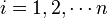
\includegraphics[scale=.6]{graphics/4a4a450cda66c931dce2ee4b3b3af329.png},
the mean is
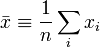
\includegraphics[scale=.6]{graphics/520b3480cda5c9ab4ab7691ae9cdd696.png},
while the stddev is
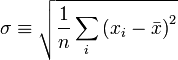
\includegraphics[scale=.6]{graphics/d678d4d0af6d46165b3712e36b9718d9.png}.

When examining a large quantity of data, one often uses a
\href{http://en.wikipedia.org/wiki/Histogram}{histogram}, which shows
the counts of data samples falling into a prechosen set of intervals (or
bins). When plotted, often as bar graphs, it visually indicates how
often each data value occurs.

\textbf{Task} Using your language's random number routine, generate real
numbers in the range of {[}0, 1{]}. It doesn't matter if you chose to
use open or closed range. Create 100 of such numbers (i.e. sample size
100) and calculate their mean and stddev. Do so for sample size of 1,000
and 10,000, maybe even higher if you feel like. Show a histogram of any
of these sets. Do you notice some patterns about the standard deviation?

\textbf{Extra} Sometimes so much data need to be processed that it's
impossible to keep all of them at once. Can you calculate the mean,
stddev and histogram of a trillion numbers? (You don't really need to do
a trillion numbers, just show how it can be done.)

\begin{description}
\item[Hint]
\end{description}

For a finite population with equal probabilities at all points, one can
derive:

\begin{figure}[H]
\centering
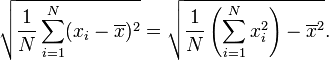
\includegraphics[scale=.6]{graphics/1a6a1cf8fdc67e4bd31e60a052c3c9ae.png}
% \caption{
% \textbackslash{}sqrt\{\textbackslash{}frac\{1\}\{N\}\textbackslash{}sum\_\{i=1\}\^{}N(x\_i-\textbackslash{}overline\{x\})\^{}2\}
% = \textbackslash{}sqrt\{\textbackslash{}frac\{1\}\{N\}
% \textbackslash{}left(\textbackslash{}sum\_\{i=1\}\^{}N
% x\_i\^{}2\textbackslash{}right) - \textbackslash{}overline\{x\}\^{}2\}.
% }
\end{figure}


\begin{wideverbatim}

The following has no limit on the number of samples. The 'statistics' function
accepts an executable body 'Prg', which it calls repeatedly to get the samples.

(scl 6)

(de statistics (Cnt . Prg)
   (prinl Cnt " numbers")
   (let (Sum 0  Sqr 0  Hist (need 10 NIL 0))
      (do Cnt
         (let N (run Prg 1)  # Get next number
            (inc 'Sum N)
            (inc 'Sqr (*/ N N 1.0))
            (inc (nth Hist (inc (/ N 0.1)))) ) )
      (let M (*/ Sum Cnt)
         (prinl "Mean:   " (round M))
         (prinl "StdDev: "
            (round
               (sqrt
                  (* 1.0
                     (- (*/ Sqr Cnt) (*/ M M 1.0)) ) ) ) ) )
      (for (I . H) Hist
         (prin (format I 1) " ")
         (do (*/ H 400 Cnt) (prin '=))
         (prinl) ) ) )

Test:

(statistics 100
   (rand 0 (dec 1.0)) )
(prinl)

(statistics 10000
   (rand 0 (dec 1.0)) )
(prinl)

(statistics 1000000
   (rand 0 (dec 1.0)) )
(prinl)


\end{wideverbatim}

\begin{wideverbatim}


Output:
100 numbers
Mean:   0.501
StdDev: 0.284
0.1 ========================================
0.2 ====================================
0.3 ====================================================
0.4 ========================
0.5 ========================
0.6 ================================================================
0.7 ========================================================
0.8 ====================================
0.9 ========================
1.0 ============================================

10000 numbers
Mean:   0.501
StdDev: 0.288
0.1 =======================================
0.2 ========================================
0.3 =======================================
0.4 =========================================
0.5 =========================================
0.6 ========================================
0.7 =========================================
0.8 ========================================
0.9 ========================================
1.0 ========================================

1000000 numbers
Mean:   0.500
StdDev: 0.289
0.1 ========================================
0.2 ========================================
0.3 ========================================
0.4 ========================================
0.5 ========================================
0.6 ========================================
0.7 ========================================
0.8 ========================================
0.9 ========================================
1.0 ========================================

\end{wideverbatim}

\pagebreak{}
\section*{Stem-and-leaf plot}

Create a well-formatted
\href{http://en.wikipedia.org/wiki/Stem-and-leaf\_plot}{stem-and-leaf
plot} from the following data set, where the leaves are the last digits:

\begin{quote}
12 127 28 42 39 113 42 18 44 118 44 37 113 124 37 48 127 36 29 31 125
139 131 115 105 132 104 123 35 113 122 42 117 119 58 109 23 105 63 27 44
105 99 41 128 121 116 125 32 61 37 127 29 113 121 58 114 126 53 114 96
25 109 7 31 141 46 13 27 43 117 116 27 7 68 40 31 115 124 42 128 52 71
118 117 38 27 106 33 117 116 111 40 119 47 105 57 122 109 124 115 43 120
43 27 27 18 28 48 125 107 114 34 133 45 120 30 127 31 116 146
\end{quote}

The primary intent of this task is the presentation of information. It
is acceptable to hardcode the data set or characteristics of it (such as
what the stems are) in the example, insofar as it is impractical to make
the example generic to any data set. For example, in a computation-less
language like HTML the data set may be entirely prearranged within the
example; the interesting characteristics are how the proper visual
formatting is arranged.

If possible, the output should not be a bitmap image.
\texttt{Monospaced plain text} is acceptable, but do better if you can.
It may be a window, i.e. not a file.

\textbf{Note:} If you wish to try multiple data sets, you might try
\emph{this generator}.


\begin{wideverbatim}

(de *Data
   12 127 28 42 39 113 42 18 44 118 44 37 113 124 37 48 127 36
   29 31 125 139 131 115 105 132 104 123 35 113 122 42 117 119
   58 109 23 105 63 27 44 105 99 41 128 121 116 125 32 61 37 127
   29 113 121 58 114 126 53 114 96 25 109 7 31 141 46 13 27 43
   117 116 27 7 68 40 31 115 124 42 128 52 71 118 117 38 27 106
   33 117 116 111 40 119 47 105 57 122 109 124 115 43 120 43 27
   27 18 28 48 125 107 114 34 133 45 120 30 127 31 116 146 )

(let L
   (group
      (mapcar
         '((N)
            (cons
               (or (format (head -1 (setq N (chop N)))) 0)
               (last N) ) )
         (sort *Data) ) )
   (for I (range (caar L) (car (last L)))
      (prinl (align 3 I) " | " (glue " " (cdr (assoc I L)))) ) )

Output:

  0 | 7 7
  1 | 2 3 8 8
  2 | 3 5 7 7 7 7 7 7 8 8 9 9
  3 | 0 1 1 1 1 2 3 4 5 6 7 7 7 8 9
  4 | 0 0 1 2 2 2 2 3 3 3 4 4 4 5 6 7 8 8
  5 | 2 3 7 8 8
  6 | 1 3 8
  7 | 1
  8 |
  9 | 6 9
 10 | 4 5 5 5 5 6 7 9 9 9
 11 | 1 3 3 3 3 4 4 4 5 5 5 6 6 6 6 7 7 7 7 8 8 9 9
 12 | 0 0 1 1 2 2 3 4 4 4 5 5 5 6 7 7 7 7 8 8
 13 | 1 2 3 9
 14 | 1 6

\end{wideverbatim}

\pagebreak{}
\section*{Straddling checkerboard}

Implement functions to encrypt and decrypt a message using the
\href{http://en.wikipedia.org/wiki/Straddling\_checkerboard}{straddling
checkerboard} method. When setting the checkerboard up, it should take a
28 character alphabet (A-Z plus a full stop and an escape character) and
two different numbers representing the blanks in the first row. The
output will be a series of decimal digits.

When encrypting, numbers should be encrypted by inserting the escape
character before each digit, then including the digit unencrypted. This
should be reversed for decryption.

\begin{wideverbatim}

(de *Straddling
   (NIL  "H"  "O"  "L"  NIL  "M"  "E"  "S"  NIL  "R"  "T")
   ("3"  "A"  "B"  "C"  "D"  "F"  "G"  "I"  "J"  "K"  "N")
   ("7"  "P"  "Q"  "U"  "V"  "W"  "X"  "Y"  "Z"  "."  "/")
   ("79" "0"  "1"  "2"  "3"  "4"  "5"  "6"  "7"  "8"  "9") )

(de straddle (Str)
   (pack
      (mapcar
         '((C)
            (pick
               '((L)
                  (and
                     (index C (cdr L))
                     (cons (car L) (dec @)) ) )
               *Straddling ) )
         (chop (uppc Str)) ) ) )

(de unStraddle (Str)
   (pack
      (make
         (for (L (chop Str)  L)
            (let C (pop 'L)
               (setq C
                  (if (assoc C *Straddling)
                     (get (cdr @) (inc (format (pop 'L))))
                     (get (cdar *Straddling) (inc (format C))) ) )
               (link (if (= "/" C) (pop 'L) C)) ) ) ) ) )

Output:

: (straddle "One night-it was on the twentieth of March, 1888-I was returning")
-> "13953936350936974306139905974539936590
    1344308320791798798798367430685972839363935"

: (unStraddle @)
-> "ONENIGHTITWASONTHETWENTIETHOFMARCH1888IWASRETURNING"

\end{wideverbatim}

\pagebreak{}
\section*{String case}

Take the string ``alphaBETA'', and demonstrate how to convert it to
UPPER-CASE and lower-case. Use the default encoding of a string literal
or plain ASCII if there is no string literal in your language. Show any
additional case conversion functions (e.g. swapping case, capitalizing
the first letter, etc.) that may be included in the library of your
language.


\begin{wideverbatim}

(let Str "alphaBETA"
   (prinl (uppc Str))
   (prinl (lowc Str)) )

\end{wideverbatim}

\pagebreak{}
\section*{String concatenation}

\textbf{Basic Data Operation}\\ This is a basic data operation. It
represents a fundamental action on a basic data type.

You may see other such operations in the
\emph{Basic Data Operations}
category, or:

\textbf{Integer Operations} \\
\emph{Arithmetic} \textbar{}
\emph{Comparison}

\textbf{Boolean Operations} \\ \emph{Bitwise}
\textbar{} \emph{Logical}

\textbf{String Operations} \\ \textbf{Concatenation} \textbar{}
\emph{Interpolation} \textbar{}
\emph{Matching}

\textbf{Memory Operations} \\
\emph{Pointers \& references}
\textbar{} \emph{Addresses}

Create a string variable equal to any text value. Create another string
variable whose value is the original variable concatenated with another
string literal.

To illustrate the operation, show the content of the variables.

\begin{wideverbatim}

(let Str1 "First text"
   (prinl Str1 " literal")
   (let Str2 (pack Str1 " literal")
      (prinl Str2) ) )

\end{wideverbatim}

\pagebreak{}
\section*{String interpolation (included)}


\textbf{Basic Data Operation}\\ This is a basic data operation. It
represents a fundamental action on a basic data type.

You may see other such operations in the
\emph{Basic Data Operations}
category, or:

\textbf{Integer Operations} \\
\emph{Arithmetic} \textbar{}
\emph{Comparison}

\textbf{Boolean Operations} \\ \emph{Bitwise}
\textbar{} \emph{Logical}

\textbf{String Operations} \\
\emph{Concatenation} \textbar{}
\textbf{Interpolation} \textbar{}
\emph{Matching}

\textbf{Memory Operations} \\
\emph{Pointers \& references}
\textbar{} \emph{Addresses}

Given a string and defined variables or values,
\href{http://en.wikipedia.org/wiki/String\_literal\#Variable\_interpolation}{string
interpolation} is the replacement of defined character sequences in the
string by values or variable values.

For example, given an original string of \texttt{"Mary had a X lamb."},
a value of ``big'', and if the language replaces X in its interpolation
routine, then the result of its interpolation would be the string
\texttt{"Mary had a big lamb"}.

(Languages usually include an infrequently used character or sequence of
characters to indicate what is to be replaced such as ``\%'', or ``\#''
rather than ``X'').

The task is to:

\begin{enumerate}
\item
  Use your languages inbuilt string interpolation abilities to
  interpolate a string missing the text \texttt{"little"} which is held
  in a variable, to produce the output string
  \texttt{"Mary had a little lamb"}.
\item
  If possible, give links to further documentation on your languages
  string interpolation features.
\end{enumerate}

Note: The task is not to create a string interpolation routine, but to
show a language's built-in capability.



\begin{wideverbatim}

(let Extra "little"
   (prinl (text "Mary had a @1 lamb." Extra)) )

\end{wideverbatim}

\pagebreak{}
\section*{String length}

In this task, the goal is to find the \emph{character} and \emph{byte}
length of a string. This means encodings like \emph{UTF-8}
need to be handled properly, as there is not necessarily a one-to-one
relationship between bytes and characters. By \emph{character}, we mean
an individual Unicode \emph{code point}, not a user-visible
\emph{grapheme} containing combining characters. For example, the
character length of ``møøse'' is 5 but the byte length is 7 in UTF-8 and
10 in UTF-16.

Non-BMP code points (those between 0x10000 and 0x10FFFF) must also be
handled correctly: answers should produce actual character counts in
code points, not in code unit counts. Therefore a string like
``𝔘𝔫𝔦𝔠𝔬𝔡𝔢'' (consisting of the 7 Unicode characters U+1D518 U+1D52B
U+1D526 U+1D520 U+1D52C U+1D521 U+1D522) is 7 characters long,
\textbf{not} 14 UTF-16 code units; and it is 28 bytes long whether
encoded in UTF-8 or in UTF-16.

Please mark your examples with ===Character Length=== or ===Byte
Length===. If your language is capable of providing the string length in
graphemes, mark those examples with ===Grapheme Length===. For example,
the string ``J̲o̲s̲é̲''
(``J\textbackslash{}x\{332\}o\textbackslash{}x\{332\}s\textbackslash{}x\{332\}e\textbackslash{}x\{301\}\textbackslash{}x\{332\}'')
has 4 user-visible graphemes, 9 characters (code points), and 14 bytes
when encoded in UTF-8.



\begin{wideverbatim}

(let Str "møøse"
   (prinl "Character Length of \"" Str "\" is " (length Str))
   (prinl "Byte Length of \"" Str "\" is " (size Str)) )

Output:

Character Length of "møøse" is 5
Byte Length of "møøse" is 7
-> 7

\end{wideverbatim}

\pagebreak{}
\section*{Strip a set of characters from a string}

The task is to create a function that strips a set of characters from a
string. The function should take two arguments: the first argument being
a string to stripped and the second, a string containing the set of
characters to be stripped. The returned string should contain the first
string, stripped of any characters in the second argument:

\begin{wideverbatim}
print stripchars("She was a soul stripper. She took my heart!","aei")
Sh ws  soul strppr. Sh took my hrt!
\end{wideverbatim}

\begin{wideverbatim}

(de strDiff (Str1 Str2)
   (pack (diff (chop Str1) (chop Str2))) )

Test:

: (strDiff "She was a soul stripper. She took my heart!" "aei")
-> "Sh ws  soul strppr. Sh took my hrt!"

\end{wideverbatim}

\pagebreak{}
\section*{Strip block comments}

A block comment begins with a \emph{beginning delimiter} and ends with a
\emph{ending delimiter}, including the delimiters. These delimiters are
often multi-character sequences.

\textbf{Task:} Strip block comments from program text (of a programming
language much like classic \emph{C}). Your demos should at
least handle simple, non-nested and multiline block comment delimiters.
The beginning delimiter is the two-character sequence ``\texttt{/*}''
and the ending delimiter is ``\texttt{*/}''.

Sample text for stripping:

\begin{verbatim}
  /**
   * Some comments
   * longer comments here that we can parse.
   *
   * Rahoo 
   */
   function subroutine() {
    a = /* inline comment */ b + c ;
   }
   /*/ <-- tricky comments */

   /**
    * Another comment.
    */
    function something() {
    }
\end{verbatim}

\textbf{Extra credit:} Ensure that the stripping code is not
hard-coded to the particular delimiters described above, but instead
allows the caller to specify them. (If your language supports them,
\emph{optional parameters} may be useful for this.)

C.f: \emph{Strip comments from a string}


\begin{wideverbatim}

(in "sample.txt"
   (while (echo "/*")
      (out "/dev/null" (echo "*/")) ) )

Output:


   function subroutine() {
    a =  b + c ;
   }



    function something() {
    }

\end{wideverbatim}

\pagebreak{}
\section*{Strip comments from a string}

The task is to remove text that follow any of a set of comment markers,
(in these examples either a hash or a semicolon) from a string or input
line.

The following examples will be truncated to either ``apples, pears'' or
``apples, pears''. (This example has flipped between ``apples, pears''
and ``apples, pears'' in the past.)

\begin{verbatim}
apples, pears # and bananas
apples, pears ; and bananas
\end{verbatim}

Cf. \emph{Strip block comments}


\begin{wideverbatim}

(for Str '("apples, pears # and bananas" "apples, pears ; and bananas")
   (prinl (car (split (chop Str) "#" ";"))) )

Output:

apples, pears
apples, pears

\end{wideverbatim}

\pagebreak{}
\section*{Strip control codes and extended characters from a string}

The task is to strip control codes and extended characters from a
string. The solution should demonstrate how to achieve each of the
following results:

\begin{itemize}
\item
  a string with control codes stripped (but extended characters not
  stripped)
\item
  a string with control codes and extended characters stripped
\end{itemize}

In ASCII, the control codes have decimal codes 0 through to 31 and 127
and greater than 126. On an ASCII based system, if the control codes are
stripped, the resultant string would have all of its characters within
the range of 32 to 126 decimal on the ascii table.

On a non-ASCII based system, we consider characters that do not have a
corresponding glyph on the ASCII table (within the ASCII range of 32 to
126 decimal) to be an extended character for the purpose of this task.


\begin{wideverbatim}

Control characters in strings are written with a hat (^) in PicoLisp.
^? is the DEL character.

(de stripCtrl (Str)
   (pack
      (filter
         '((C)
            (nor (= "^?" C) (> " " C "^A")) )
         (chop Str) ) ) )

(de stripCtrlExt (Str)
   (pack
      (filter
         '((C) (> "^?" C "^_"))
         (chop Str) ) ) )

Test:

: (char "^?")
-> 127

: (char "^_")
-> 31

: (stripCtrl "^I^M a b c^? d äöüß")
-> " a b c d äöüß"

: (stripCtrlExt "^I^M a b c^? d äöüß")
-> " a b c d "

\end{wideverbatim}

\pagebreak{}
\section*{Strip whitespace from a string/Top and tail}

The task is to demonstrate how to strip leading and trailing whitespace
from a string. The solution should demonstrate how to achieve the
following three results:

\begin{itemize}
\item
  String with leading whitespace removed
\item
  String with trailing whitespace removed
\item
  String with both leading and trailing whitespace removed
\end{itemize}

For the purposes of this task whitespace includes non printable
characters such as the space character, the tab character, and other
such characters that have no corresponding graphical representation.


\begin{wideverbatim}

(de trimLeft (Str)
   (pack (flip (trim (flip (chop Str))))) )

(de trimRight (Str)
   (pack (trim (chop Str))) )

(de trimBoth (Str)
   (pack (clip (chop Str))) )

Test:

: (trimLeft " ^G ^I trimmed left ^L ")
-> "trimmed left ^L "

: (trimRight " ^G ^I trimmed right ^L ")
-> " ^G ^I trimmed right"

: (trimBoth " ^G ^I trimmed both ^L ")
-> "trimmed both"

\end{wideverbatim}

\pagebreak{}
\section*{Subset sum problem}

Implement a function/procedure/method/subroutine that takes a
\emph{set |array | list | stream | table | collection} of words with
integer weights, and identifies a non-empty subset of them whose
weights sum to zero (cf. the Dropbox
\href{http://www.dropbox.com/jobs/challenges}{Diet} candidate
screening exercise and the
\href{http://en.wikipedia.org/wiki/Subset\_sum\_problem}{Subset sum
  problem} Wikipedia article).

For example, for this set of weighted words, one solution would be the
set of words \{elysee, efferent, deploy, departure, centipede, bonnet,
balm, archbishop\}, because their respective weights of -326, 54, 44,
952, -658, 452, 397, and -915 sum to zero.

\ctable[caption = { Table of weighted words },
pos = H, center, botcap]{ll}
{% notes
}
{% rows
\FL
word & weight
\ML
alliance & -624
\\\noalign{\medskip}
archbishop & -915
\\\noalign{\medskip}
balm & 397
\\\noalign{\medskip}
bonnet & 452
\\\noalign{\medskip}
brute & 870
\\\noalign{\medskip}
centipede & -658
\\\noalign{\medskip}
cobol & 362
\\\noalign{\medskip}
covariate & 590
\\\noalign{\medskip}
departure & 952
\\\noalign{\medskip}
deploy & 44
\\\noalign{\medskip}
diophantine & 645
\\\noalign{\medskip}
efferent & 54
\\\noalign{\medskip}
elysee & -326
\\\noalign{\medskip}
eradicate & 376
\\\noalign{\medskip}
escritoire & 856
\\\noalign{\medskip}
exorcism & -983
\\\noalign{\medskip}
fiat & 170
\\\noalign{\medskip}
filmy & -874
\\\noalign{\medskip}
flatworm & 503
\\\noalign{\medskip}
gestapo & 915
\\\noalign{\medskip}
infra & -847
\\\noalign{\medskip}
isis & -982
\\\noalign{\medskip}
lindholm & 999
\\\noalign{\medskip}
markham & 475
\\\noalign{\medskip}
mincemeat & -880
\\\noalign{\medskip}
moresby & 756
\\\noalign{\medskip}
mycenae & 183
\\\noalign{\medskip}
plugging & -266
\\\noalign{\medskip}
smokescreen & 423
\\\noalign{\medskip}
speakeasy & -745
\\\noalign{\medskip}
vein & 813
\LL
}

Another solution would be the set of words \{flatworm, gestapo, infra,
isis, lindholm, plugging, smokescreen, speakeasy\}, because their
respective weights of 503, 915, -847, -982, 999, -266, 423, and -745
also sum to zero.

You may assume the weights range from -1000 to 1000. If there are
multiple solutions, only one needs to be found. Use any algorithm you
want and demonstrate it on a set of at least 30 weighted words with the
results shown in a human readable form. Note that an implementation that
depends on enumerating all possible subsets is likely to be infeasible.

\begin{wideverbatim}

(de *Words
   (alliance . -624) (archbishop . -915) (balm . 397) (bonnet . 452)
   (brute . 870) (centipede . -658) (cobol . 362) (covariate . 590)
   (departure . 952) (deploy . 44) (diophantine . 645) (efferent . 54)
   (elysee . -326) (eradicate . 376) (escritoire . 856) (exorcism . -983)
   (fiat . 170) (filmy . -874) (flatworm . 503) (gestapo . 915)
   (infra . -847) (isis . -982) (lindholm . 999) (markham . 475)
   (mincemeat . -880) (moresby . 756) (mycenae . 183) (plugging . -266)
   (smokescreen . 423) (speakeasy . -745) (vein . 813) )

Minimal brute force solution:

(load "@lib/simul.l")  # For 'subsets'

(pick
   '((N)
      (find '((L) (=0 (sum cdr L)))
         (subsets N *Words) ) )
   (range 1 (length *Words)) )

Output:

-> ((archbishop . -915) (gestapo . 915))

\end{wideverbatim}

\pagebreak{}
\section*{Substring}

\textbf{Basic Data Operation}\\ This is a basic data operation. It
represents a fundamental action on a basic data type.

You may see other such operations in the
\emph{Basic Data Operations}
category, or:

\textbf{Integer Operations} \\
\emph{Arithmetic} \textbar{}
\emph{Comparison}

\textbf{Boolean Operations} \\ \emph{Bitwise}
\textbar{} \emph{Logical}

\textbf{String Operations} \\
\emph{Concatenation} \textbar{}
\emph{Interpolation} \textbar{}
\emph{Matching}

\textbf{Memory Operations} \\
\emph{Pointers \& references}
\textbar{} \emph{Addresses}

In this task display a substring:

\begin{itemize}
\item
  starting from \texttt{n} characters in and of \texttt{m} length;
\item
  starting from \texttt{n} characters in, up to the end of the string;
\item
  whole string minus last character;
\item
  starting from a known character within the string and of \texttt{m}
  length;
\item
  starting from a known substring within the string and of \texttt{m}
  length.
\end{itemize}

If the program uses UTF-8 or UTF-16, it must work on any valid Unicode
code point, whether in the Basic Multilingual Plane or above it. The
program must reference logical characters (code points), not 8-bit code
units for UTF-8 or 16-bit code units for UTF-16. Programs for other
encodings (such as 8-bit ASCII, or EUC-JP) are not required to handle
all Unicode characters.


\begin{wideverbatim}

(let Str (chop "This is a string")
   (prinl (head 4 (nth Str 6)))        # From 6 of 4 length
   (prinl (nth Str 6))                 # From 6 up to the end
   (prinl (head -1 Str))               # Minus last character
   (prinl (head 8 (member "s" Str)))   # From character "s" of length 8
   (prinl                              # From "isa" of length 8
      (head 8
         (seek '((S) (pre? "is a" S)) Str) ) ) )

Output:

is a
is a string
This is a strin
s is a s
is a str

\end{wideverbatim}

\pagebreak{}
\section*{Subtractive generator}

A \emph{subtractive generator} calculates a sequence of \emph{random
  numbers}, where each number is congruent to the subtraction of two
previous numbers from the sequence. The formula is

\begin{itemize}
\item
  \emph{r}\textsubscript{\emph{n}} = \emph{r}\textsubscript{(\emph{n} −
  \emph{i})} − \emph{r}\textsubscript{(\emph{n} − \emph{j})}(mod
  \emph{m})
\end{itemize}

for some fixed values of \emph{i}, \emph{j} and \emph{m}, all positive
integers. Supposing that \emph{i} \textgreater{} \emph{j}, then the
state of this generator is the list of the previous numbers from
\emph{r}\textsubscript{\emph{n} − \emph{i}} to
\emph{r}\textsubscript{\emph{n} − 1}. Many states generate uniform
random integers from 0 to \emph{m} − 1, but some states are bad. A
state, filled with zeros, generates only zeros. If \emph{m} is even,
then a state, filled with even numbers, generates only even numbers.
More generally, if \emph{f} is a factor of \emph{m}, then a state,
filled with multiples of \emph{f}, generates only multiples of \emph{f}.

All subtractive generators have some weaknesses. The formula correlates
\emph{r}\textsubscript{\emph{n}}, \emph{r}\textsubscript{(\emph{n} −
\emph{i})} and \emph{r}\textsubscript{(\emph{n} − \emph{j})}; these
three numbers are not independent, as true random numbers would be.
Anyone who observes \emph{i} consecutive numbers can predict the next
numbers, so the generator is not cryptographically secure. The authors
of \emph{Freeciv}
(\href{http://svn.gna.org/viewcvs/freeciv/trunk/utility/rand.c?view=markup}{utility/rand.c})
and \emph{xpat2} (src/testit2.c) knew another problem: the low bits are
less random than the high bits.

The subtractive generator has a better reputation than the
\emph{linear congruential
generator}, perhaps because it holds more state. A subtractive generator
might never multiply numbers: this helps where multiplication is slow. A
subtractive generator might also avoid division: the value of
\emph{r}\textsubscript{(\emph{n} − \emph{i})} −
\emph{r}\textsubscript{(\emph{n} − \emph{j})} is always between −
\emph{m} and \emph{m}, so a program only needs to add \emph{m} to
negative numbers.

The choice of \emph{i} and \emph{j} affects the period of the generator.
A popular choice is \emph{i} = 55 and \emph{j} = 24, so the formula is

\begin{itemize}
\item
  \emph{r}\textsubscript{\emph{n}} = \emph{r}\textsubscript{(\emph{n} −
  55)} − \emph{r}\textsubscript{(\emph{n} − 24)}(mod \emph{m})
\end{itemize}

The subtractive generator from \emph{xpat2} uses

\begin{itemize}
\item
  \emph{r}\textsubscript{\emph{n}} = \emph{r}\textsubscript{(\emph{n} −
  55)} − \emph{r}\textsubscript{(\emph{n} − 24)}(mod
  10\textsuperscript{9})
\end{itemize}

The implementation is by J. Bentley and comes from
program\_tools/universal.c of
\href{ftp://dimacs.rutgers.edu/pub/netflow/}{the DIMACS (netflow)
archive} at Rutgers University. It credits Knuth,
\href{http://en.wikipedia.org/wiki/The\_Art\_of\_Computer\_Programming}{\emph{TAOCP}},
Volume 2, Section 3.2.2 (Algorithm A).

\pagebreak{}
Bentley uses this clever algorithm to seed the generator.

\begin{enumerate}
\item
  Start with a single \emph{s}\emph{e}\emph{e}\emph{d} in range 0 to
  10\textsuperscript{9} − 1.
\item
  Set \emph{s}\textsubscript{0} = \emph{s}\emph{e}\emph{e}\emph{d} and
  \emph{s}\textsubscript{1} = 1. The inclusion of
  \emph{s}\textsubscript{1} = 1 avoids some bad states (like all zeros,
  or all multiples of 10).
\item
  Compute
  \emph{s}\textsubscript{2},\emph{s}\textsubscript{3},\ldots{},\emph{s}\textsubscript{54}
  using the subtractive formula \emph{s}\textsubscript{\emph{n}} =
  \emph{s}\textsubscript{(\emph{n} − 2)} −
  \emph{s}\textsubscript{(\emph{n} − 1)}(mod 10\textsuperscript{9}).
\item
  Reorder these 55 values so \emph{r}\textsubscript{0} =
  \emph{s}\textsubscript{34}, \emph{r}\textsubscript{1} =
  \emph{s}\textsubscript{13}, \emph{r}\textsubscript{2} =
  \emph{s}\textsubscript{47}, \ldots{}, \emph{r}\textsubscript{\emph{n}}
  = \emph{s}\textsubscript{(34 * (\emph{n} + 1)(mod 55))}.

  \begin{itemize}
  \item
    This is the same order as \emph{s}\textsubscript{0} =
    \emph{r}\textsubscript{54}, \emph{s}\textsubscript{1} =
    \emph{r}\textsubscript{33}, \emph{s}\textsubscript{2} =
    \emph{r}\textsubscript{12}, \ldots{},
    \emph{s}\textsubscript{\emph{n}} = \emph{r}\textsubscript{((34 *
    \emph{n}) − 1(mod 55))}.
  \item
    This rearrangement exploits how 34 and 55 are relatively prime.
  \end{itemize}
\item
  Compute the next 165 values \emph{r}\textsubscript{55} to
  \emph{r}\textsubscript{219}. Store the last 55 values.
\end{enumerate}

This generator yields the sequence \emph{r}\textsubscript{220},
\emph{r}\textsubscript{221}, \emph{r}\textsubscript{222} and so on. For
example, if the seed is 292929, then the sequence begins with
\emph{r}\textsubscript{220} = 467478574, \emph{r}\textsubscript{221} =
512932792, \emph{r}\textsubscript{222} = 539453717. By starting at
\emph{r}\textsubscript{220}, this generator avoids a bias from the first
numbers of the sequence. This generator must store the last 55 numbers
of the sequence, so to compute the next
\emph{r}\textsubscript{\emph{n}}. Any array or list would work; a
\href{/mw/index.php?title=Ring\_buffer\&action=edit\&redlink=1}{ring
buffer} is ideal but not necessary.

Implement a subtractive generator that replicates the sequences from
\emph{xpat2}.



\begin{wideverbatim}

Using a circular list (as a true "ring" buffer).

(setq
   *Bentley (apply circ (need 55))
   *Bentley2 (nth *Bentley 32) )

(de subRandSeed (S)
   (let (N 1  P (nth *Bentley 55))
      (set P S)
      (do 54
         (set (setq P (nth P 35)) N)
         (when (lt0 (setq N (- S N)))
            (inc 'N 1000000000) )
         (setq S (car P)) ) )
   (do 165 (subRand)) )

(de subRand ()
   (when (lt0 (dec *Bentley (pop '*Bentley2)))
      (inc *Bentley 1000000000) )
   (pop '*Bentley) )

Test:

(subRandSeed 292929)
(do 7 (println (subRand)))

Output:

467478574
512932792
539453717
20349702
615542081
378707948
933204586

\end{wideverbatim}

\pagebreak{}
\section*{Sudoku}

Solve a partially filled-in normal 9x9
\href{http://en.wikipedia.org/wiki/Sudoku}{Sudoku} grid and display the
result in a human-readable format.
\href{http://en.wikipedia.org/wiki/Algorithmics\_of\_sudoku}{Algorithmics
of Sudoku} may help implement this.

\begin{wideverbatim}

(load "lib/simul.l")

### Fields/Board ###
# val lst

(setq
   *Board (grid 9 9)
   *Fields (apply append *Board) )

# Init values to zero (empty)
(for L *Board
   (for This L
      (=: val 0) ) )

# Build lookup lists
(for (X . L) *Board
   (for (Y . This) L
      (=: lst
         (make
            (let A (* 3 (/ (dec X) 3))
               (do 3
                  (inc 'A)
                  (let B (* 3 (/ (dec Y) 3))
                     (do 3
                        (inc 'B)
                        (unless (and (= A X) (= B Y))
                           (link
                              (prop (get *Board A B) 'val) ) ) ) ) ) )
            (for Dir '(`west `east `south `north)
               (for (This (Dir This)  This  (Dir This))
                  (unless (memq (:: val) (made))
                     (link (:: val)) ) ) ) ) ) ) )

\end{wideverbatim}

\begin{wideverbatim}


# Cut connections (for display only)
(for (X . L) *Board
   (for (Y . This) L
      (when (member X (3 6))
         (con (car (val This))) )
      (when (member Y (4 7))
         (set (cdr (val This))) ) ) )

# Display board
(de display ()
   (disp *Board 0
      '((This)
         (if (=0 (: val))
            "   "
            (pack " " (: val) " ") ) ) ) )

# Initialize board
(de main (Lst)
   (for (Y . L) Lst
      (for (X . N) L
         (put *Board X (- 10 Y) 'val N) ) )
   (display) )

# Find solution
(de go ()
   (unless
      (recur (*Fields)
         (with (car *Fields)
            (if (=0 (: val))
               (loop
                  (NIL
                     (or
                        (assoc (inc (:: val)) (: lst))
                        (recurse (cdr *Fields)) ) )
                  (T (= 9 (: val)) (=: val 0)) )
               (recurse (cdr *Fields)) ) ) )
      (display) ) )

(main
   (quote
      (5 3 0 0 7 0 0 0 0)
      (6 0 0 1 9 5 0 0 0)
      (0 9 8 0 0 0 0 6 0)
      (8 0 0 0 6 0 0 0 3)
      (4 0 0 8 0 3 0 0 1)
      (7 0 0 0 2 0 0 0 6)
      (0 6 0 0 0 0 2 8 0)
      (0 0 0 4 1 9 0 0 5)
      (0 0 0 0 8 0 0 7 9) ) )

\end{wideverbatim}

\begin{wideverbatim}


Output:

   +---+---+---+---+---+---+---+---+---+
 9 | 5   3     |     7     |           |
   +   +   +   +   +   +   +   +   +   +
 8 | 6         | 1   9   5 |           |
   +   +   +   +   +   +   +   +   +   +
 7 |     9   8 |           |     6     |
   +---+---+---+---+---+---+---+---+---+
 6 | 8         |     6     |         3 |
   +   +   +   +   +   +   +   +   +   +
 5 | 4         | 8       3 |         1 |
   +   +   +   +   +   +   +   +   +   +
 4 | 7         |     2     |         6 |
   +---+---+---+---+---+---+---+---+---+
 3 |     6     |           | 2   8     |
   +   +   +   +   +   +   +   +   +   +
 2 |           | 4   1   9 |         5 |
   +   +   +   +   +   +   +   +   +   +
 1 |           |     8     |     7   9 |
   +---+---+---+---+---+---+---+---+---+
     a   b   c   d   e   f   g   h   i

(go)
   +---+---+---+---+---+---+---+---+---+
 9 | 5   3   4 | 6   7   8 | 9   1   2 |
   +   +   +   +   +   +   +   +   +   +
 8 | 6   7   2 | 1   9   5 | 3   4   8 |
   +   +   +   +   +   +   +   +   +   +
 7 | 1   9   8 | 3   4   2 | 5   6   7 |
   +---+---+---+---+---+---+---+---+---+
 6 | 8   5   9 | 7   6   1 | 4   2   3 |
   +   +   +   +   +   +   +   +   +   +
 5 | 4   2   6 | 8   5   3 | 7   9   1 |
   +   +   +   +   +   +   +   +   +   +
 4 | 7   1   3 | 9   2   4 | 8   5   6 |
   +---+---+---+---+---+---+---+---+---+
 3 | 9   6   1 | 5   3   7 | 2   8   4 |
   +   +   +   +   +   +   +   +   +   +
 2 | 2   8   7 | 4   1   9 | 6   3   5 |
   +   +   +   +   +   +   +   +   +   +
 1 | 3   4   5 | 2   8   6 | 1   7   9 |
   +---+---+---+---+---+---+---+---+---+
     a   b   c   d   e   f   g   h   i

\end{wideverbatim}

\pagebreak{}
\section*{Sum and product of an array}

Compute the sum and product of an array of integers.

\begin{wideverbatim}

(let Data (1 2 3 4 5)
   (cons
      (apply + Data)
      (apply * Data) ) )

Output:

(15 . 120)

\end{wideverbatim}

\pagebreak{}
\section*{Sum digits of an integer}

This task takes a Natural Number in a given Base and returns the sum of
it digits:

$1_{10}$ sums to $1$;

$1234_{10}$ sums to $10$;

$fe_{16}$ sums to $29$;

$f0e_{16}$ sums to $29$.


\begin{wideverbatim}

(de sumDigits (N Base)
   (or
      (=0 N)
      (+ (\% N Base) (sumDigits (/ N Base) Base)) ) )

Test:

: (sumDigits 1 10)
-> 1

: (sumDigits 1234 10)
-> 10

: (sumDigits (hex "fe") 16)
-> 29

: (sumDigits (hex "f0e") 16)
-> 29

\end{wideverbatim}

\pagebreak{}
\section*{Sum of a series}

Compute the \emph{n}th partial sum of a series.

For this task, use S(x) = 1/x\textsuperscript{2}, from 1 to 1000. (This
approximates the Riemann zeta function. The Basel problem solved this:
$\zeta(2) = \pi\textsuperscript{2}/6$.)

\begin{wideverbatim}

(scl 9)  # Calculate with 9 digits precision

(let S 0
   (for I 1000
      (inc 'S (*/ 1.0 (* I I))) )
   (prinl (round S 6)) )  # Round result to 6 digits

1.643935

\end{wideverbatim}

\pagebreak{}
\section*{Sum of squares}

Write a program to find the sum of squares of a numeric vector. The
program should work on a zero-length vector (with an answer of 0).

See also \emph{Mean}.


\begin{wideverbatim}

: (sum '((N) (* N N)) (3 1 4 1 5 9))
-> 133
: (sum '((N) (* N N)) ())
-> 0

\end{wideverbatim}

\pagebreak{}
\section*{Symmetric difference}


Given two \emph{sets} \emph{A} and \emph{B}, where \emph{A}
contains:

\begin{itemize}
\item
  John
\item
  Bob
\item
  Mary
\item
  Serena
\end{itemize}

and \emph{B} contains:

\begin{itemize}
\item
  Jim
\item
  Mary
\item
  John
\item
  Bob
\end{itemize}

compute

\begin{figure}[H]
\centering
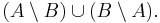
\includegraphics[scale=.6]{graphics/cd81bcd600dda401fc4cfbc6646bbbc9.png}
% \caption{(A \textbackslash{}setminus B) \textbackslash{}cup (B
% \textbackslash{}setminus A).}
\end{figure}

That is, enumerate the items that are in \emph{A} or \emph{B} but not
both. This set is called the
\href{http://en.wikipedia.org/wiki/Symmetric\_difference}{symmetric
difference} of \emph{A} and \emph{B}.

In other words:
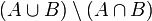
\includegraphics[scale=.6]{graphics/3fdf48da32bf746ea787b61406ca05e7.png}
(the set of items that are in at least one of \emph{A} or \emph{B} minus
the set of items that are in both \emph{A} and \emph{B}).

Optionally, give the individual differences
( 
\includegraphics[scale=.6]{graphics/2958d3ea0159c6ad2ed45f5804fce621.png}
and  
 
\includegraphics[scale=.6]{graphics/07915cb82d7470aff79636e93397abe3.png})
as well.

Notes

\begin{enumerate}
\item If your code uses lists of items to represent sets then ensure
  duplicate items in lists are correctly handled. For example two
  lists representing sets of \texttt{a = {[}"John", "Serena", "Bob",
    "Mary", }\texttt{"Serena"{]}} and \texttt{b = {[}"Jim", "Mary",
    "John", "Jim", "Bob"{]}} should produce the result of just two
  strings: \texttt{{[}"Serena", "Jim"{]}}, in any order.
\item
  In the mathematical notation above \texttt{A \textbackslash{} B} gives
  the set of items in A that are not in B; \texttt{A ∪ B} gives the set
  of items in both A and B, (their \emph{union}); and \texttt{A ∩ B}
  gives the set of items that are in both A and B (their
  \emph{intersection}).
\end{enumerate}



\begin{wideverbatim}

(de symdiff (A B)
   (uniq (conc (diff A B) (diff B A))) )

Output:

(symdiff '(John Serena Bob Mary Serena) '(Jim Mary John Jim Bob))
-> (Serena Jim)

\end{wideverbatim}

\pagebreak{}
\section*{Synchronous concurrency}


The goal of this task is to create two concurrent activities
("\emph{Threads}" or ``Tasks'', not \emph{processes}.) that share data
synchronously. Your language may provide syntax or libraries to
perform concurrency. Different languages provide different
implementations of concurrency, often with different names. Some
languages use the term threads, others use the term tasks, while
others use co-processes. This task should not be implemented using
fork, spawn, or the \emph{Linux}/\emph{UNIX}/\emph{Win32} pipe
command, as communication should be between threads, not processes.

One of the concurrent units will read from a file named ``input.txt''
and send the contents of that file, one line at a time, to the other
concurrent unit, which will print the line it receives to standard
output. The printing unit must count the number of lines it prints.
After the concurrent unit reading the file sends its last line to the
printing unit, the reading unit will request the number of lines printed
by the printing unit. The reading unit will then print the number of
lines printed by the printing unit.

This task requires two-way communication between the concurrent units.
All concurrent units must cleanly terminate at the end of the program.


\begin{wideverbatim}

PicoLisp has no threads, but synchronous background tasks and asynchronous
signal handlers, or coroutines.

# Using background tasks and signals

The following two tasks communicate via UDP, so in fact they don't need to run
within the same process and not even the same machine. "input.txt" would rather
be a device (like a named pipe or socket) than a plain file.

# Reading task (synchronous)
(task (open "input.txt")
   (let Fd @
      (if (in Fd (line T))             # More lines?
         (udp "localhost" 4444 @)      # Yes: Send next line
         (task (port T 4445)           # Else install handler
            (prinl (udp @) " lines")   # to receive and print count
            (task (close @)) )
         (udp "localhost" 4444 T)      # Send 'T' for "Done"
         (task (close Fd)) ) ) )       # Stop the task

# Printing task (asynchronous)
(sigio (setq "Sock" (port T 4444))
   (job '((Cnt . 0))
      (let? X (udp "Sock")
         (if (=T X)                    # Done?
            (prog
               (udp "localhost" 4445 Cnt) # Yes: Send count
               (sigio (close "Sock")) )   # and stop the task
            (println X)                # Else print line to stdout
            (inc 'Cnt) ) ) ) )         # and increment count

# Using coroutines

Coroutines are available only in the 64-bit version.

(co 'unit1
   (yield)                       # Allow 'unit2' to start
   (in "input.txt"               # Read the file
      (while (line T)            # Send each line
         (yield @ 'unit2) ) )    # to 'unit2'
   (prinl
      (yield NIL 'unit2)         # Send 'NIL' for "Done", receive count
      " lines" ) )

(co 'unit2
   (let Cnt 0                    # Init counter
      (while (yield NIL 'unit1)  # Receive line
         (println @)             # Print it
         (inc 'Cnt) )            # Increment count
      (yield Cnt 'unit1) ) )     # Send count to 'unit1'

\end{wideverbatim}

\pagebreak{}
\section*{System time}

Output the system time (any units will do as long as they are noted)
either by a \emph{system command} or
one built into the language. The system time can be used for debugging,
network information, random number seeds, or something as simple as
program performance.

\textbf{See Also}

\begin{itemize}
\item
  \emph{Date format}
\item
  \href{http://en.wikipedia.org/wiki/System\_time\#Retrieving\_system\_time}{Retrieving
  system time (wiki)}
\end{itemize}


\begin{wideverbatim}

(stamp)

Output:

-> "2010-02-19 15:14:06"

\end{wideverbatim}



% %%%%%%%%%%%%%%%%%%%%%%%% referenc.tex %%%%%%%%%%%%%%%%%%%%%%%%%%%%%%
% sample references
% %
% Use this file as a template for your own input.
%
%%%%%%%%%%%%%%%%%%%%%%%% Springer-Verlag %%%%%%%%%%%%%%%%%%%%%%%%%%
%
% BibTeX users please use
% \bibliographystyle{}
% \bibliography{}
%
\biblstarthook{In view of the parallel print and (chapter-wise) online publication of your book at \url{www.springerlink.com} it has been decided that -- as a genreral rule --  references should be sorted chapter-wise and placed at the end of the individual chapters. However, upon agreement with your contact at Springer you may list your references in a single seperate chapter at the end of your book. Deactivate the class option \texttt{sectrefs} and the \texttt{thebibliography} environment will be put out as a chapter of its own.\\\indent
References may be \textit{cited} in the text either by number (preferred) or by author/year.\footnote{Make sure that all references from the list are cited in the text. Those not cited should be moved to a separate \textit{Further Reading} section or chapter.} The reference list should ideally be \textit{sorted} in alphabetical order -- even if reference numbers are used for the their citation in the text. If there are several works by the same author, the following order should be used: 
\begin{enumerate}
\item all works by the author alone, ordered chronologically by year of publication
\item all works by the author with a coauthor, ordered alphabetically by coauthor
\item all works by the author with several coauthors, ordered chronologically by year of publication.
\end{enumerate}
The \textit{styling} of references\footnote{Always use the standard abbreviation of a journal's name according to the ISSN \textit{List of Title Word Abbreviations}, see \url{http://www.issn.org/en/node/344}} depends on the subject of your book:
\begin{itemize}
\item The \textit{two} recommended styles for references in books on \textit{mathematical, physical, statistical and computer sciences} are depicted in ~\cite{science-contrib, science-online, science-mono, science-journal, science-DOI} and ~\cite{phys-online, phys-mono, phys-journal, phys-DOI, phys-contrib}.
\item Examples of the most commonly used reference style in books on \textit{Psychology, Social Sciences} are~\cite{psysoc-mono, psysoc-online,psysoc-journal, psysoc-contrib, psysoc-DOI}.
\item Examples for references in books on \textit{Humanities, Linguistics, Philosophy} are~\cite{humlinphil-journal, humlinphil-contrib, humlinphil-mono, humlinphil-online, humlinphil-DOI}.
\item Examples of the basic Springer style used in publications on a wide range of subjects such as \textit{Computer Science, Economics, Engineering, Geosciences, Life Sciences, Medicine, Biomedicine} are ~\cite{basic-contrib, basic-online, basic-journal, basic-DOI, basic-mono}. 
\end{itemize}
}

\begin{thebibliography}{99.}%
% and use \bibitem to create references.
%
% Use the following syntax and markup for your references if 
% the subject of your book is from the field 
% "Mathematics, Physics, Statistics, Computer Science"
%
% Contribution 
\bibitem{science-contrib} Broy, M.: Software engineering --- from auxiliary to key technologies. In: Broy, M., Dener, E. (eds.) Software Pioneers, pp. 10-13. Springer, Heidelberg (2002)
%
% Online Document
\bibitem{science-online} Dod, J.: Effective substances. In: The Dictionary of Substances and Their Effects. Royal Society of Chemistry (1999) Available via DIALOG. \\
\url{http://www.rsc.org/dose/title of subordinate document. Cited 15 Jan 1999}
%
% Monograph
\bibitem{science-mono} Geddes, K.O., Czapor, S.R., Labahn, G.: Algorithms for Computer Algebra. Kluwer, Boston (1992) 
%
% Journal article
\bibitem{science-journal} Hamburger, C.: Quasimonotonicity, regularity and duality for nonlinear systems of partial differential equations. Ann. Mat. Pura. Appl. \textbf{169}, 321--354 (1995)
%
% Journal article by DOI
\bibitem{science-DOI} Slifka, M.K., Whitton, J.L.: Clinical implications of dysregulated cytokine production. J. Mol. Med. (2000) doi: 10.1007/s001090000086 
%
\bigskip

% Use the following (APS) syntax and markup for your references if 
% the subject of your book is from the field 
% "Mathematics, Physics, Statistics, Computer Science"
%
% Online Document
\bibitem{phys-online} J. Dod, in \textit{The Dictionary of Substances and Their Effects}, Royal Society of Chemistry. (Available via DIALOG, 1999), 
\url{http://www.rsc.org/dose/title of subordinate document. Cited 15 Jan 1999}
%
% Monograph
\bibitem{phys-mono} H. Ibach, H. L\"uth, \textit{Solid-State Physics}, 2nd edn. (Springer, New York, 1996), pp. 45-56 
%
% Journal article
\bibitem{phys-journal} S. Preuss, A. Demchuk Jr., M. Stuke, Appl. Phys. A \textbf{61}
%
% Journal article by DOI
\bibitem{phys-DOI} M.K. Slifka, J.L. Whitton, J. Mol. Med., doi: 10.1007/s001090000086
%
% Contribution 
\bibitem{phys-contrib} S.E. Smith, in \textit{Neuromuscular Junction}, ed. by E. Zaimis. Handbook of Experimental Pharmacology, vol 42 (Springer, Heidelberg, 1976), p. 593
%
\bigskip
%
% Use the following syntax and markup for your references if 
% the subject of your book is from the field 
% "Psychology, Social Sciences"
%
%
% Monograph
\bibitem{psysoc-mono} Calfee, R.~C., \& Valencia, R.~R. (1991). \textit{APA guide to preparing manuscripts for journal publication.} Washington, DC: American Psychological Association.
%
% Online Document
\bibitem{psysoc-online} Dod, J. (1999). Effective substances. In: The dictionary of substances and their effects. Royal Society of Chemistry. Available via DIALOG. \\
\url{http://www.rsc.org/dose/Effective substances.} Cited 15 Jan 1999.
%
% Journal article
\bibitem{psysoc-journal} Harris, M., Karper, E., Stacks, G., Hoffman, D., DeNiro, R., Cruz, P., et al. (2001). Writing labs and the Hollywood connection. \textit{J Film} Writing, 44(3), 213--245.
%
% Contribution 
\bibitem{psysoc-contrib} O'Neil, J.~M., \& Egan, J. (1992). Men's and women's gender role journeys: Metaphor for healing, transition, and transformation. In B.~R. Wainrig (Ed.), \textit{Gender issues across the life cycle} (pp. 107--123). New York: Springer.
%
% Journal article by DOI
\bibitem{psysoc-DOI}Kreger, M., Brindis, C.D., Manuel, D.M., Sassoubre, L. (2007). Lessons learned in systems change initiatives: benchmarks and indicators. \textit{American Journal of Community Psychology}, doi: 10.1007/s10464-007-9108-14.
%
%
% Use the following syntax and markup for your references if 
% the subject of your book is from the field 
% "Humanities, Linguistics, Philosophy"
%
\bigskip
%
% Journal article
\bibitem{humlinphil-journal} Alber John, Daniel C. O'Connell, and Sabine Kowal. 2002. Personal perspective in TV interviews. \textit{Pragmatics} 12:257--271
%
% Contribution 
\bibitem{humlinphil-contrib} Cameron, Deborah. 1997. Theoretical debates in feminist linguistics: Questions of sex and gender. In \textit{Gender and discourse}, ed. Ruth Wodak, 99--119. London: Sage Publications.
%
% Monograph
\bibitem{humlinphil-mono} Cameron, Deborah. 1985. \textit{Feminism and linguistic theory.} New York: St. Martin's Press.
%
% Online Document
\bibitem{humlinphil-online} Dod, Jake. 1999. Effective substances. In: The dictionary of substances and their effects. Royal Society of Chemistry. Available via DIALOG. \\
http://www.rsc.org/dose/title of subordinate document. Cited 15 Jan 1999
%
% Journal article by DOI
\bibitem{humlinphil-DOI} Suleiman, Camelia, Daniel C. O�Connell, and Sabine Kowal. 2002. `If you and I, if we, in this later day, lose that sacred fire...�': Perspective in political interviews. \textit{Journal of Psycholinguistic Research}. doi: 10.1023/A:1015592129296.
%
%
%
\bigskip
%
%
% Use the following syntax and markup for your references if 
% the subject of your book is from the field 
% "Computer Science, Economics, Engineering, Geosciences, Life Sciences"
%
%
% Contribution 
\bibitem{basic-contrib} Brown B, Aaron M (2001) The politics of nature. In: Smith J (ed) The rise of modern genomics, 3rd edn. Wiley, New York 
%
% Online Document
\bibitem{basic-online} Dod J (1999) Effective Substances. In: The dictionary of substances and their effects. Royal Society of Chemistry. Available via DIALOG. \\
\url{http://www.rsc.org/dose/title of subordinate document. Cited 15 Jan 1999}
%
% Journal article by DOI
\bibitem{basic-DOI} Slifka MK, Whitton JL (2000) Clinical implications of dysregulated cytokine production. J Mol Med, doi: 10.1007/s001090000086
%
% Journal article
\bibitem{basic-journal} Smith J, Jones M Jr, Houghton L et al (1999) Future of health insurance. N Engl J Med 965:325--329
%
% Monograph
\bibitem{basic-mono} South J, Blass B (2001) The future of modern genomics. Blackwell, London 
%
\end{thebibliography}

